% Options for packages loaded elsewhere
\PassOptionsToPackage{unicode}{hyperref}
\PassOptionsToPackage{hyphens}{url}
%
\documentclass[
]{article}
\usepackage{amsmath,amssymb}
\usepackage{iftex}
\ifPDFTeX
  \usepackage[T1]{fontenc}
  \usepackage[utf8]{inputenc}
  \usepackage{textcomp} % provide euro and other symbols
\else % if luatex or xetex
  \usepackage{unicode-math} % this also loads fontspec
  \defaultfontfeatures{Scale=MatchLowercase}
  \defaultfontfeatures[\rmfamily]{Ligatures=TeX,Scale=1}
\fi
\usepackage{lmodern}
\ifPDFTeX\else
  % xetex/luatex font selection
\fi
% Use upquote if available, for straight quotes in verbatim environments
\IfFileExists{upquote.sty}{\usepackage{upquote}}{}
\IfFileExists{microtype.sty}{% use microtype if available
  \usepackage[]{microtype}
  \UseMicrotypeSet[protrusion]{basicmath} % disable protrusion for tt fonts
}{}
\makeatletter
\@ifundefined{KOMAClassName}{% if non-KOMA class
  \IfFileExists{parskip.sty}{%
    \usepackage{parskip}
  }{% else
    \setlength{\parindent}{0pt}
    \setlength{\parskip}{6pt plus 2pt minus 1pt}}
}{% if KOMA class
  \KOMAoptions{parskip=half}}
\makeatother
\usepackage{xcolor}
\usepackage[margin=1in]{geometry}
\usepackage{color}
\usepackage{fancyvrb}
\newcommand{\VerbBar}{|}
\newcommand{\VERB}{\Verb[commandchars=\\\{\}]}
\DefineVerbatimEnvironment{Highlighting}{Verbatim}{commandchars=\\\{\}}
% Add ',fontsize=\small' for more characters per line
\usepackage{framed}
\definecolor{shadecolor}{RGB}{248,248,248}
\newenvironment{Shaded}{\begin{snugshade}}{\end{snugshade}}
\newcommand{\AlertTok}[1]{\textcolor[rgb]{0.94,0.16,0.16}{#1}}
\newcommand{\AnnotationTok}[1]{\textcolor[rgb]{0.56,0.35,0.01}{\textbf{\textit{#1}}}}
\newcommand{\AttributeTok}[1]{\textcolor[rgb]{0.13,0.29,0.53}{#1}}
\newcommand{\BaseNTok}[1]{\textcolor[rgb]{0.00,0.00,0.81}{#1}}
\newcommand{\BuiltInTok}[1]{#1}
\newcommand{\CharTok}[1]{\textcolor[rgb]{0.31,0.60,0.02}{#1}}
\newcommand{\CommentTok}[1]{\textcolor[rgb]{0.56,0.35,0.01}{\textit{#1}}}
\newcommand{\CommentVarTok}[1]{\textcolor[rgb]{0.56,0.35,0.01}{\textbf{\textit{#1}}}}
\newcommand{\ConstantTok}[1]{\textcolor[rgb]{0.56,0.35,0.01}{#1}}
\newcommand{\ControlFlowTok}[1]{\textcolor[rgb]{0.13,0.29,0.53}{\textbf{#1}}}
\newcommand{\DataTypeTok}[1]{\textcolor[rgb]{0.13,0.29,0.53}{#1}}
\newcommand{\DecValTok}[1]{\textcolor[rgb]{0.00,0.00,0.81}{#1}}
\newcommand{\DocumentationTok}[1]{\textcolor[rgb]{0.56,0.35,0.01}{\textbf{\textit{#1}}}}
\newcommand{\ErrorTok}[1]{\textcolor[rgb]{0.64,0.00,0.00}{\textbf{#1}}}
\newcommand{\ExtensionTok}[1]{#1}
\newcommand{\FloatTok}[1]{\textcolor[rgb]{0.00,0.00,0.81}{#1}}
\newcommand{\FunctionTok}[1]{\textcolor[rgb]{0.13,0.29,0.53}{\textbf{#1}}}
\newcommand{\ImportTok}[1]{#1}
\newcommand{\InformationTok}[1]{\textcolor[rgb]{0.56,0.35,0.01}{\textbf{\textit{#1}}}}
\newcommand{\KeywordTok}[1]{\textcolor[rgb]{0.13,0.29,0.53}{\textbf{#1}}}
\newcommand{\NormalTok}[1]{#1}
\newcommand{\OperatorTok}[1]{\textcolor[rgb]{0.81,0.36,0.00}{\textbf{#1}}}
\newcommand{\OtherTok}[1]{\textcolor[rgb]{0.56,0.35,0.01}{#1}}
\newcommand{\PreprocessorTok}[1]{\textcolor[rgb]{0.56,0.35,0.01}{\textit{#1}}}
\newcommand{\RegionMarkerTok}[1]{#1}
\newcommand{\SpecialCharTok}[1]{\textcolor[rgb]{0.81,0.36,0.00}{\textbf{#1}}}
\newcommand{\SpecialStringTok}[1]{\textcolor[rgb]{0.31,0.60,0.02}{#1}}
\newcommand{\StringTok}[1]{\textcolor[rgb]{0.31,0.60,0.02}{#1}}
\newcommand{\VariableTok}[1]{\textcolor[rgb]{0.00,0.00,0.00}{#1}}
\newcommand{\VerbatimStringTok}[1]{\textcolor[rgb]{0.31,0.60,0.02}{#1}}
\newcommand{\WarningTok}[1]{\textcolor[rgb]{0.56,0.35,0.01}{\textbf{\textit{#1}}}}
\usepackage{graphicx}
\makeatletter
\def\maxwidth{\ifdim\Gin@nat@width>\linewidth\linewidth\else\Gin@nat@width\fi}
\def\maxheight{\ifdim\Gin@nat@height>\textheight\textheight\else\Gin@nat@height\fi}
\makeatother
% Scale images if necessary, so that they will not overflow the page
% margins by default, and it is still possible to overwrite the defaults
% using explicit options in \includegraphics[width, height, ...]{}
\setkeys{Gin}{width=\maxwidth,height=\maxheight,keepaspectratio}
% Set default figure placement to htbp
\makeatletter
\def\fps@figure{htbp}
\makeatother
\setlength{\emergencystretch}{3em} % prevent overfull lines
\providecommand{\tightlist}{%
  \setlength{\itemsep}{0pt}\setlength{\parskip}{0pt}}
\setcounter{secnumdepth}{-\maxdimen} % remove section numbering
\renewcommand{\contentsname}{Sumário}
\usepackage{booktabs}
\usepackage{longtable}
\usepackage{array}
\usepackage{multirow}
\usepackage{wrapfig}
\usepackage{float}
\usepackage{colortbl}
\usepackage{pdflscape}
\usepackage{tabu}
\usepackage{threeparttable}
\usepackage{threeparttablex}
\usepackage[normalem]{ulem}
\usepackage{makecell}
\usepackage{xcolor}
\usepackage{siunitx}

  \newcolumntype{d}{S[
    input-open-uncertainty=,
    input-close-uncertainty=,
    parse-numbers = false,
    table-align-text-pre=false,
    table-align-text-post=false
  ]}
  
\ifLuaTeX
  \usepackage{selnolig}  % disable illegal ligatures
\fi
\IfFileExists{bookmark.sty}{\usepackage{bookmark}}{\usepackage{hyperref}}
\IfFileExists{xurl.sty}{\usepackage{xurl}}{} % add URL line breaks if available
\urlstyle{same}
\hypersetup{
  pdftitle={Análise descritiva para dados de nascidos vivos diagnosticados com anomalia congênita - 11-20},
  hidelinks,
  pdfcreator={LaTeX via pandoc}}

\title{Análise descritiva para dados de nascidos vivos diagnosticados
com anomalia congênita - 11-20}
\author{}
\date{\vspace{-2.5em}}

\begin{document}
\maketitle

{
\setcounter{tocdepth}{1}
\tableofcontents
}
Neste relatório, será apresentada uma análise exploratória dos
microdrados de anomalias congênitas obtidos das bases do Sistema de
Informações sobre Nascidos Vivos (SINASC), previamente tratadas pela
PCDaS com base no fluxo ETL (Extract, Transform e Load). Para a extração
dos microdados, foram considerados todos os casos datados de 2011 a 2020
em que \texttt{IDANOMAL\ =\ 1\ (Sim)} ou existia alguma resposta válida
para \texttt{CODANOMAL}.

As bases são providas do portal openDataSUS, mantido pelo Ministério da
Saúde.

\newpage

\hypertarget{dicionuxe1rio-das-variuxe1veis}{%
\section{1. Dicionário das
variáveis}\label{dicionuxe1rio-das-variuxe1veis}}

Nesta seção, encontra-se o dicionário das variáveis que compõem as bases
de dados do Sistema de Informações sobre Nascidos Vivos (SINASC)
tratadas pela PCDaS.

Para as análises subsequentes, foram selecionados somente os casos em
que o recém-nascido (RN) foi registrado com pelo menos uma CID-10 que
faz parte do Capítulo XVII. Malformações congênitas, deformidades e
anomalias cromossômicas (Q000-Q999) \textbf{ou} com a CID-10 D180, cuja
descrição é hemangioma de qualquer localização.

\begin{Shaded}
\begin{Highlighting}[]
\NormalTok{d\_anom }\OtherTok{\textless{}{-}}\NormalTok{ readr}\SpecialCharTok{::}\FunctionTok{read\_csv}\NormalTok{(}\StringTok{"01.dados/anomalias/microdados\_ac\_11{-}20.csv"}\NormalTok{) }\SpecialCharTok{|\textgreater{}} 
  \CommentTok{\# selecionando anos de 2011 a 2020 e apenas cids do capitulo xvii + d180}
  \FunctionTok{filter}\NormalTok{(}
    \FunctionTok{as.numeric}\NormalTok{(ano\_nasc) }\SpecialCharTok{\textgreater{}} \DecValTok{2010}\NormalTok{,}
    \FunctionTok{str\_detect}\NormalTok{(CODANOMAL, }\StringTok{"Q"}\NormalTok{) }\SpecialCharTok{|} \FunctionTok{str\_detect}\NormalTok{(CODANOMAL, }\StringTok{"D180"}\NormalTok{)}
\NormalTok{ )}
\end{Highlighting}
\end{Shaded}

Sob as condições mencionadas, isto é, quando
\texttt{IDANOMAL\ =\ 1\ (Sim)} ou existia alguma resposta válida para
\texttt{CODANOMAL} e o RN foi registrado com ao menos uma CID-10 contida
no Capítulo XVII ou com a CID-10 D180, foram coletadas 240405
observações para as quais haviam ou não informações em \textbf{135
variáveis}. São elas:

\hypertarget{variuxe1veis-sinasc}{%
\subsection{Variáveis SINASC}\label{variuxe1veis-sinasc}}

\begin{itemize}
\tightlist
\item
  \textbf{\ldots1}: Índice
\item
  \textbf{APGAR1}: Apgar no primeiro minuto 00 a 10
\item
  \textbf{APGAR5}: Apgar no quinto minuto 00 a 10
\item
  \textbf{CODANOMAL}: Código de malformação congênita ou anomalia
  cromossômica, de acordo com a CID-10
\item
  \textbf{CODBAINASC}: Código do bairro de nascimento
\item
  \textbf{CODBAIRES}: Código do bairro de residência
\item
  \textbf{CODCART}: Código de Cartório
\item
  \textbf{CODESTAB}: Código do estabelecimento onde ocorreu o nascimento
\item
  \textbf{CODINST}: Código da Instalação da geração dos Registros
\item
  \textbf{CODMUNCART}: Código do município do cartório
\item
  \textbf{CODMUNNASC}: Município de ocorrência, em codificação idêntica
  a de CODMUNRES, conforme tabela TABMUN
\item
  \textbf{CODMUNNATU}: Código do município de naturalidade da mãe
\item
  \textbf{CODMUNRES}: Município de residência da mãe, em codificação
  idêntica a de CODMUNNASC, conforme tabela TABMUN
\item
  \textbf{CODOCUPMAE}: Ocupação, conforme a Classificação Brasileira de
  Ocupações (CBO-2002)
\item
  \textbf{CODPAISRES}: Código do país de residência
\item
  \textbf{CODUFNATU}: Código da UF de naturalidade da mãe
\item
  \textbf{CODPAISRES}: Código do país de residência
\item
  \textbf{CODUFNATU}: Código da UF de naturalidade da mãe
\item
  \textbf{CONSPRENAT}: Número de consultas pré‐natal
\item
  \textbf{CONSULTAS}: Número de consultas de pré-natal: 1: Nenhuma; 2:
  de 1 a 3; 3: de 4 a 6; 4: 7 e mais; 9: Ignorado
\item
  \textbf{CONTADOR}: Número identificador do registro
\item
  \textbf{CODPAISRES}: Código do país de residência
\item
  \textbf{CODUFNATU}: Código da UF de naturalidade da mãe
\item
  \textbf{CONSPRENAT}: Número de consultas pré‐natal
\item
  \textbf{CONSULTAS}: Número de consultas de pré-natal: 1: Nenhuma; 2:
  de 1 a 3; 3: de 4 a 6; 4: 7 e mais; 9: Ignorado
\item
  \textbf{CONTADOR}: Número identificador do registro
\item
  \textbf{DIFDATA}: Diferença entre a data de Nascimento e data do
  recebimento original da DN ({[}DTNASC{]} - {[}DTRECORIGA{]})
\item
  \textbf{DTCADASTRO}: Data do cadastro da DN no sistema
\item
  \textbf{DTDECLARAC}: Data da declaração: dd mm aaaa
\item
  \textbf{DTNASC}: Data do nascimento, no formato ddmmaaaa
\item
  \textbf{DTNASCMAE}: Data de nascimento da mãe
\item
  \textbf{DTRECEBIM}: Data de recebimento no nível central, data da
  última atualização do registro
\item
  \textbf{DTRECORIG}: Data do primeiro recebimento do lote, dada pelo
  Sisnet
\item
  \textbf{DTRECORIGA}: Cria-se campo DTRECORIGA e copia os valores de
  DTRECORIG para esse campo. Se DTRECORIGA = Nulo, copia os valores de
  DTRECEBIM. Se DTRECEBIM = Nulo, copia os valores de DTCADASTRO
\item
  \textbf{DTREGCART}: Data do registro do cartório
\item
  \textbf{DTULTMENST}: Data da última menstruação (DUM): dd mm aaaa
\item
  \textbf{ESCMAE}: Escolaridade, anos de estudo concluídos: 1: Nenhuma;
  2: 1 a 3 anos; 3: 4 a 7 anos; 4: 8 a 11 anos; 5: 12 e mais; 9:
  Ignorado
\item
  \textbf{ESCMAE2010}: Escolaridade 2010. Valores: 0 - Sem escolaridade;
  1 - Fundamental I (1a a 4a série); 2 - Fundamental II (5a a 8a série);
  3 - Médio (antigo 2o Grau); 4 - Superior incompleto; 5 - Superior
  completo; 9 - Ignorado
\item
  \textbf{ESCMAEAGR1}: Escolaridade 2010 agregada. Valores: 00 - Sem
  Escolaridade; 01 - Fundamental I Incompleto; 02 - Fundamental I
  Completo; 03 - Fundamental II Incompleto; 04 - Fundamental II
  Completo; 05 - Ensino Médio Incompleto; 06 - Ensino Médio Completo; 07
  - Superior Incompleto; 08 - Superior Completo; 09 - Ignorado; 10 --
  Fundamental I Incompleto ou Inespecífico; 11 - Fundamental II
  Incompleto ou Inespecífico; 12 - Ensino Médio Incompleto ou
  Inespecífico
\item
  \textbf{ESTCIVMAE}: Estado civil, conforme a tabela: 1: Solteira; 2:
  Casada; 3: Viuva; 4: Separado judicialmente/Divorciado; 5: União
  consensual (versões anteriores); 9: Ignorado
\item
  \textbf{GESTACAO}: Semanas de gestação, conforme a tabela: 9:
  Ignorado; 1: Menos de 22 semanas; 2: 22 a 27 semanas; 3: 28 a 31
  semanas; 4: 32 a 36 semanas; 5: 37 a 41 semanas; 6: 42 semanas e mais
\item
  \textbf{GRAVIDEZ}: Tipo de gravidez, conforme a tabela: 9: Ignorado;
  1: Única; 2: Dupla; 3: Tripla e mais
\item
  \textbf{HORANASC}: Horário de nascimento
\item
  \textbf{IDADEMAE}: Idade da mãe em anos
\item
  \textbf{IDADEPAI}: Idade do pai
\item
  \textbf{IDANOMAL}: Anomalia congênita: 9: Ignorado; 1: Sim; 2: Não
\item
  \textbf{KOTELCHUCK}: Índice de Kotelchuck - Avaliação de assistência
  pré-natal
\item
  \textbf{LOCNASC}: Local de ocorrência do nascimento, conforme a
  tabela: 9: Ignorado; 1: Hospital; 2: Outro Estab Saúde; 3: Domicílio;
  4: Outros
\item
  \textbf{MESPRENAT}: Mês de gestação em que iniciou o pré‐natal
\item
  \textbf{NATURALMAE}: Se a mãe for estrangeira, constará o código do
  país de nascimento
\item
  \textbf{NOVO}: -
\item
  \textbf{NUMERODN}: Número da DN, sequencial por UF informante e por
  ano
\item
  \textbf{NUMEROLOTE}: Número do lote
\item
  \textbf{NUMREGCART}: Número do Registro do Cartório
\item
  \textbf{ORIGEM}: Banco de dados de Origem 1 Oracle, 2 FTP, 3 - SEAD
\item
  \textbf{PARIDADE}: Define se é a primeira gravidez ou se teve mais de
  uma. 1 - Multípara; 0 - Nulípara
\item
  \textbf{PARTO}: Tipo de parto, conforme a tabela: 9: Ignorado; 1:
  Vaginal; 2: Cesáreo
\item
  \textbf{PESO}: Peso ao nascer, em gramas
\item
  \textbf{PREFIXODN}: Prefixo da DN
\item
  \textbf{QTDFILMORT}: Número de filhos mortos
\item
  \textbf{QTDFILVIVO}: Número de filhos vivos
\item
  \textbf{QTDGESTANT}: Número de gestações anteriores
\item
  \textbf{QTDPARTCES}: Número de partos cesáreos
\item
  \textbf{QTDPARTNOR}: Número de partos vaginais
\item
  \textbf{RACACOR}: Raça/Cor da mãe: 1: Branca; 2: Preta; 3: Amarela; 4:
  Parda; 5: Indígena
\item
  \textbf{RACACOR\_RN}: Tipo de raça e cor do nascido: 1 - Branca; 2 -
  Preta; 3 - Amarela; 4 - Parda; 5 - Indígena
\item
  \textbf{SEMAGESTAC}: Número de semanas de gestação
\item
  \textbf{SERIESCMAE}: Série escolar da mãe. Valores de 1 a 8
\item
  \textbf{SEXO}: Sexo, conforme a tabela: 0: Ignorado, não informado; 1:
  Masculino; 2: Feminino
\item
  \textbf{STCESPARTO}: Cesárea ocorreu antes do trabalho de parto
  iniciar? Valores: 1 - Sim; 2 - Não; 3 - Não se aplica; 9 - Ignorado
\item
  \textbf{STDNEPIDEM}: Status de DO Epidemiológica. Valores: 1 - SIM; 0
  - NÃO
\item
  \textbf{STDNNOVA}: Status de DO Nova. Valores: 1 - SIM; 0 - NÃO
\item
  \textbf{STTRABPART}: Trabalho de parto induzido? Valores: 1 - Sim; 2 -
  Não; 3 - Não se aplica; 9 - Ignorado
\item
  \textbf{TPAPRESENT}: Tipo de apresentação do RN. Valores: 1 -
  Cefálico; 2 - Pélvica ou podálica; 3 - Transversa; 9 - Ignorado
\item
  \textbf{TPDOCRESP}: Tipo do documento do responsável. Valores: 1 -
  CNES; 2 - CRM; 3 - COREN; 4 - RG; 5 - CPF
\item
  \textbf{TPFUNCRESP}: Tipo de função do responsável pelo preenchimento.
  Valores:1 - Médico; 2 - Enfermeiro; 3 - Parteira; 4 - Funcionário
  docartório; 5 - Outros
\item
  \textbf{TPMETESTIM}: Método utilizado. Valores: 1 - Exame físico; 2 -
  Outro método; 9 - Ignorado
\item
  \textbf{TPNASCASSI}: Nascimento foi assistido por? Valores: 1 -
  Médico; 2 - Enfermeira/obstetriz; 3 - Parteira; 4 - Outros; 9 -
  Ignorado
\item
  \textbf{TPROBSON}: Código do Grupo de Robson, gerado pelo sistema
\item
  \textbf{UFINFORM}: Código da UF que informou o registro
\item
  \textbf{VERSAOSIST}: Versão do sistema
\end{itemize}

\hypertarget{variuxe1veis-pcdas}{%
\subsection{Variáveis PCDaS}\label{variuxe1veis-pcdas}}

\begin{itemize}
\tightlist
\item
  \textbf{ano\_nasc}: Ano do nascimento
\item
  \textbf{codanomal\_capitulo}: Capítulo CID-10 da malformação congênita
  ou anomalia cromossômica
\item
  \textbf{codanomal\_categoria}: Categoria CID-10 da malformação
  congênita ou anomalia cromossômica
\item
  \textbf{codanomal\_grupo}: Grupo CID-10 da malformação congênita ou
  anomalia cromossômica
\item
  \textbf{codanomal\_subcategoria}: Subcategoria CID-10 da malformação
  congênita ou anomalia cromossômica
\item
  \textbf{contador}: -
\item
  \textbf{data\_nasc}: Data de nascimento
\item
  \textbf{def\_anomalia}: Anomalia congênita (Ignorado; Sim; Não)
\item
  \textbf{def\_consultas}: Número de consultas durante o pré-natal
  (Nenhuma; de 1 a 3; de 4 a 6; 7 e mais; Ignorado)
\item
  \textbf{def\_escol\_mae}: Escolaridade da mãe (Nenhuma; de 1 a 3 anos;
  de 4 a 7 anos; 8 a 11 anos; 12 anos e mais; Ignorado)
\item
  \textbf{def\_est\_civil}: Estado civil (Situação conjugal: Solteiro;
  Casado; Viúvo; Separado judicialmente/divorciado; União estável;
  Ignorado)
\item
  \textbf{def\_gestacao}: Semana de gestação (Nominal, com as seguintes
  classificações: Menos de 22 semanas; 22 a 27 semanas; 28 a 31 semanas;
  32 a 36 semanas; 37 a 41 semanas; 42 semanas ou mais)
\item
  \textbf{def\_gravidez}: Tipo de gravidez (Nominal, com as seguintes
  classificações: Única; Dupla; Tripla e mais e Ignorada)
\item
  \textbf{def\_loc\_nasc}: Local de nascimento (Nominal, com as
  seguintes classificações: Hospital; Outros estabelecimentos de saúde;
  Domicílio; Via pública; Outros; Ignorado)
\item
  \textbf{def\_parto}: Tipo de parto (Nominal, com as seguintes
  classificações: Vaginal; Cesáreo; Ignorado)
\item
  \textbf{def\_parto\_prematuro}: Indica a prematuridade do nascimento.
  Termo: não há indícios de prematuridade; Inconclusivo-IG: há indício
  de prematuridade dado pela idade gestacional
  (\texttt{GESTACAO\textless{}=4}); Inconclusivo-Peso: há indício de
  prematuridade dado pelo peso ao nascer (\texttt{PESO\textless{}2500});
  Prematuro: a idade gestacional e o peso ao nascer indicam
  prematuridade
\item
  \textbf{def\_raca\_cor}: Raça/cor do nascido (Nominal, com as
  seguintes classificações: Branca; Preta; Amarela; Parda; Indígena)
\item
  \textbf{def\_sexo}: Sexo (Nominal, com as seguintes classificações:
  Masculino; Feminino; Ignorado)
\item
  \textbf{dia\_semana\_nasc}: Dia da semana em que ocorreu o nascimento
  (dom; seg; ter; qua; qui; sex; sáb)
\item
  \textbf{nasc\_ALTITUDE}: Altitude do município de nascimento
\item
  \textbf{nasc\_AMAZONIA}: Indica (S/N) se o município de nascimento faz
  parte da Amazônia Legal (conforme IBGE)
\item
  \textbf{nasc\_AREA}: Área do município de nascimento
\item
  \textbf{nasc\_CAPITAL}: Indica (S/N) se o município de nascimento é
  capital de UF
\item
  \textbf{nasc\_CODIGO\_UF}: Código da UF de nascimento
\item
  \textbf{nasc\_CSAUDCOD}: Código da Microrregional de Saúde a que o
  Município de nascimento pertence
\item
  \textbf{nasc\_FRONTEIRA}: Indica (S/N) se o município de nascimento
  faz parte da faixa de fronteira (conforme IBGE)
\item
  \textbf{nasc\_LATITUDE}: Latitude do município de nascimento
\item
  \textbf{nasc\_LONGITUDE}: Longitude do município de nascimento
\item
  \textbf{nasc\_MSAUDCOD}: Código da Macrorregional de Saúde a que o
  Município de nascimento pertence
\item
  \textbf{nasc\_MUNNOME}: Nome do município de nascimento
\item
  \textbf{nasc\_MUNNOMEX}: Nome do município de nascimento em maiúsculas
  e sem acentos
\item
  \textbf{nasc\_NOME\_UF}: Nome da unidade da federação de nascimento
\item
  \textbf{nasc\_REGIAO}: Nome da região da unidade da federação de
  nascimento
\item
  \textbf{nasc\_RSAUDCOD}: Código da Regional de Saúde a que o Município
  de nascimento pertence
\item
  \textbf{nasc\_SIGLA\_UF}: Sigla da unidade da federação de nascimento
\item
  \textbf{nasc\_codigo\_adotado}: Armazena o código atribuído ao
  município de nascimento atualmente, tratando os casos em que múltiplos
  códigos tenham sido utilizados para um mesmo município ao longo do
  tempo
\item
  \textbf{nasc\_coordenadas}: Coordenadas do município de nascimento
\item
  \textbf{parto\_prematuro}: Indica a prematuridade do nascimento. 0:
  não há indícios de prematuridade; 1: há indício de prematuridade dado
  pela idade gestacional (\texttt{GESTACAO\textless{}=4}); 2: há indício
  de prematuridade dado pelo peso ao nascer
  (\texttt{PESO\textless{}2500}); 3: a idade gestacional e o peso ao
  nascer indicam prematuridade
\item
  \textbf{res\_ALTITUDE}: Altitude do município de residência
\item
  \textbf{res\_AMAZONIA}: Indica (S/N) se o município de residência faz
  parte da Amazônia Legal (conforme IBGE)
\item
  \textbf{res\_ANOEXT}: -
\item
  \textbf{res\_AREA}: Área do município de residência
\item
  \textbf{res\_CAPITAL}: Indica (S/N) se o município de residência é
  capital de UF
\item
  \textbf{res\_CODIGO\_UF}: Código da UF de residência
\item
  \textbf{res\_CSAUDCOD}: Código da Microrregional de Saúde a que o
  Município de residência pertence
\item
  \textbf{res\_FRONTEIRA}: Indica (S/N) se o município de residência faz
  parte da faixa de fronteira (conforme IBGE)
\item
  \textbf{res\_LATITUDE}: Latitude do município de residência
\item
  \textbf{res\_LONGITUDE}: Longitude do município de residência
\item
  \textbf{res\_MSAUDCOD}: Código da Macrorregional de Saúde a que o
  Município de residência pertence
\item
  \textbf{res\_MUNNOME}: Nome do município de residência
\item
  \textbf{res\_MUNNOMEX}: Nome do município de residência em maiúsculas
  e sem acentos
\item
  \textbf{res\_NOME\_UF}: Nome da unidade da federação de residência
\item
  \textbf{res\_REGIAO}: Nome da região da unidade da federação de
  residência
\item
  \textbf{res\_RSAUDCOD}: Código da Regional de Saúde a que o Município
  de residência pertence
\item
  \textbf{res\_SIGLA\_UF}: Sigla da unidade da federação de residência
\item
  \textbf{res\_SUCESSOR}: -
\item
  \textbf{res\_codigo\_adotado}: Armazena o código atribuído ao
  município de residência atualmente, tratando os casos em que múltiplos
  códigos tenham sido utilizados para um mesmo município ao longo do
  tempo
\item
  \textbf{res\_coordenadas}: Coordenadas do município de residência
\end{itemize}

\newpage

\hypertarget{manipulauxe7uxe3o-dos-dados}{%
\section{2. Manipulação dos dados}\label{manipulauxe7uxe3o-dos-dados}}

Nesta seção, foi feita uma breve higienização dos dados a fim de melhor
manipulá-los.

\hypertarget{transformando-valores-99-e-categoria-ignorado-em-nas}{%
\subsubsection{Transformando valores 99 e categoria `ignorado' em
NAs}\label{transformando-valores-99-e-categoria-ignorado-em-nas}}

\begin{Shaded}
\begin{Highlighting}[]
\NormalTok{d\_anom }\OtherTok{\textless{}{-}}\NormalTok{ d\_anom }\SpecialCharTok{|\textgreater{}}  
  \FunctionTok{mutate}\NormalTok{(}
    \AttributeTok{CONSPRENAT =} \FunctionTok{as.numeric}\NormalTok{(}\FunctionTok{ifelse}\NormalTok{(CONSPRENAT }\SpecialCharTok{==} \DecValTok{99}\NormalTok{, }\ConstantTok{NA\_character\_}\NormalTok{, CONSPRENAT)),}
    \AttributeTok{IDADEMAE =} \FunctionTok{as.numeric}\NormalTok{(}\FunctionTok{ifelse}\NormalTok{(IDADEMAE }\SpecialCharTok{==} \DecValTok{99}\NormalTok{, }\ConstantTok{NA\_character\_}\NormalTok{, IDADEMAE)),}
    \AttributeTok{IDADEPAI =} \FunctionTok{as.numeric}\NormalTok{(}\FunctionTok{ifelse}\NormalTok{(IDADEPAI }\SpecialCharTok{==} \DecValTok{99}\NormalTok{, }\ConstantTok{NA\_character\_}\NormalTok{, IDADEPAI)),}
    \AttributeTok{KOTELCHUCK =} \FunctionTok{as.numeric}\NormalTok{(}\FunctionTok{ifelse}\NormalTok{(KOTELCHUCK }\SpecialCharTok{==} \DecValTok{9}\NormalTok{, }\ConstantTok{NA\_character\_}\NormalTok{, KOTELCHUCK)),}
    \AttributeTok{MESPRENAT =} \FunctionTok{as.numeric}\NormalTok{(}\FunctionTok{ifelse}\NormalTok{(MESPRENAT }\SpecialCharTok{==} \DecValTok{99}\NormalTok{, }\ConstantTok{NA\_character\_}\NormalTok{, MESPRENAT)),}
    \AttributeTok{PESO =} \FunctionTok{as.numeric}\NormalTok{(}\FunctionTok{ifelse}\NormalTok{(PESO }\SpecialCharTok{==} \DecValTok{9999}\NormalTok{, }\ConstantTok{NA\_character\_}\NormalTok{, PESO)),}
    \AttributeTok{QTDFILMORT =} \FunctionTok{as.numeric}\NormalTok{(}\FunctionTok{ifelse}\NormalTok{(QTDFILMORT }\SpecialCharTok{==} \DecValTok{99}\NormalTok{, }\ConstantTok{NA\_character\_}\NormalTok{, QTDFILMORT)),}
    \AttributeTok{QTDFILVIVO =} \FunctionTok{as.numeric}\NormalTok{(}\FunctionTok{ifelse}\NormalTok{(QTDFILVIVO }\SpecialCharTok{==} \DecValTok{99}\NormalTok{, }\ConstantTok{NA\_character\_}\NormalTok{, QTDFILVIVO)),}
    \AttributeTok{QTDGESTANT =} \FunctionTok{as.numeric}\NormalTok{(}\FunctionTok{ifelse}\NormalTok{(QTDGESTANT }\SpecialCharTok{==} \DecValTok{99}\NormalTok{, }\ConstantTok{NA\_character\_}\NormalTok{, QTDGESTANT)),}
    \AttributeTok{QTDPARTCES =} \FunctionTok{as.numeric}\NormalTok{(}\FunctionTok{ifelse}\NormalTok{(QTDPARTCES }\SpecialCharTok{==} \DecValTok{99}\NormalTok{, }\ConstantTok{NA\_character\_}\NormalTok{, QTDPARTCES)),}
    \AttributeTok{QTDPARTNOR =} \FunctionTok{as.numeric}\NormalTok{(}\FunctionTok{ifelse}\NormalTok{(QTDPARTNOR }\SpecialCharTok{==} \DecValTok{99}\NormalTok{, }\ConstantTok{NA\_character\_}\NormalTok{, QTDPARTNOR)),}
    \AttributeTok{def\_anomalia =} \FunctionTok{ifelse}\NormalTok{(def\_anomalia }\SpecialCharTok{==} \StringTok{"Ignorado"}\NormalTok{, }\ConstantTok{NA\_character\_}\NormalTok{, def\_anomalia),}
    \AttributeTok{def\_consultas =} \FunctionTok{ifelse}\NormalTok{(def\_consultas }\SpecialCharTok{==} \StringTok{"Ignorado"}\NormalTok{, }\ConstantTok{NA\_character\_}\NormalTok{, def\_consultas),}
    \AttributeTok{def\_escol\_mae =} \FunctionTok{ifelse}\NormalTok{(def\_escol\_mae }\SpecialCharTok{==} \StringTok{"Ignorado"}\NormalTok{, }\ConstantTok{NA\_character\_}\NormalTok{, def\_escol\_mae),}
    \AttributeTok{def\_est\_civil =} \FunctionTok{ifelse}\NormalTok{(def\_est\_civil }\SpecialCharTok{==} \StringTok{"Ignorado"}\NormalTok{, }\ConstantTok{NA\_character\_}\NormalTok{, def\_est\_civil),}
    \AttributeTok{def\_gestacao =} \FunctionTok{ifelse}\NormalTok{(def\_gestacao }\SpecialCharTok{==} \StringTok{"Ignorado"}\NormalTok{, }\ConstantTok{NA\_character\_}\NormalTok{, def\_gestacao),}
    \AttributeTok{def\_gravidez =} \FunctionTok{ifelse}\NormalTok{(def\_gravidez }\SpecialCharTok{==} \StringTok{"Ignorado"}\NormalTok{, }\ConstantTok{NA\_character\_}\NormalTok{, def\_gravidez),}
    \AttributeTok{def\_loc\_nasc =} \FunctionTok{ifelse}\NormalTok{(def\_loc\_nasc }\SpecialCharTok{==} \StringTok{"Ignorado"}\NormalTok{, }\ConstantTok{NA\_character\_}\NormalTok{, def\_loc\_nasc),}
    \AttributeTok{def\_parto =} \FunctionTok{ifelse}\NormalTok{(def\_parto }\SpecialCharTok{==} \StringTok{"Ignorado"}\NormalTok{, }\ConstantTok{NA\_character\_}\NormalTok{, def\_parto),}
    \AttributeTok{def\_parto\_prematuro =} \FunctionTok{ifelse}\NormalTok{(def\_parto\_prematuro }\SpecialCharTok{==} \StringTok{"Ignorado"}\NormalTok{, }\ConstantTok{NA\_character\_}\NormalTok{,}
\NormalTok{                                   def\_parto\_prematuro),}
    \AttributeTok{def\_raca\_cor =} \FunctionTok{ifelse}\NormalTok{(def\_raca\_cor }\SpecialCharTok{==} \StringTok{"Ignorado"}\NormalTok{, }\ConstantTok{NA\_character\_}\NormalTok{, def\_raca\_cor),}
    \AttributeTok{def\_sexo =} \FunctionTok{ifelse}\NormalTok{(def\_sexo }\SpecialCharTok{==} \StringTok{"Ignorado"}\NormalTok{, }\ConstantTok{NA\_character\_}\NormalTok{, def\_sexo),}
    \AttributeTok{TPROBSON =} \FunctionTok{ifelse}\NormalTok{((d\_anom}\SpecialCharTok{$}\NormalTok{TPROBSON }\SpecialCharTok{==} \DecValTok{11} \SpecialCharTok{|}\NormalTok{ d\_anom}\SpecialCharTok{$}\NormalTok{TPROBSON }\SpecialCharTok{==} \DecValTok{12}\NormalTok{),}
                         \ConstantTok{NA\_character\_}\NormalTok{, d\_anom}\SpecialCharTok{$}\NormalTok{TPROBSON)}
\NormalTok{ )}
\end{Highlighting}
\end{Shaded}

\hypertarget{separando-casos-em-que-o-nascido-tem-mais-de-uma-malformauxe7uxe3o-conguxeanita}{%
\subsubsection{Separando casos em que o nascido tem mais de uma
malformação
congênita}\label{separando-casos-em-que-o-nascido-tem-mais-de-uma-malformauxe7uxe3o-conguxeanita}}

\begin{Shaded}
\begin{Highlighting}[]
\NormalTok{d\_anom }\OtherTok{\textless{}{-}}\NormalTok{ d\_anom }\SpecialCharTok{\%\textgreater{}\%}
  \FunctionTok{separate}\NormalTok{(}
\NormalTok{    ., }\AttributeTok{col =}\NormalTok{ CODANOMAL, }
    \AttributeTok{into =} \FunctionTok{c}\NormalTok{(}\StringTok{"coda1"}\NormalTok{, }\StringTok{"coda2"}\NormalTok{, }\StringTok{"coda3"}\NormalTok{, }\StringTok{"coda4"}\NormalTok{, }\StringTok{"coda5"}\NormalTok{, }\StringTok{"coda6"}\NormalTok{), }\AttributeTok{sep =} \StringTok{"Q"}\NormalTok{, }
    \AttributeTok{remove =} \ConstantTok{FALSE}
\NormalTok{  ) }\SpecialCharTok{|\textgreater{}}
  \CommentTok{\# incluindo na nas celulas vazias das cids}
  \FunctionTok{mutate}\NormalTok{(}
    \AttributeTok{coda1 =} \FunctionTok{ifelse}\NormalTok{(coda1 }\SpecialCharTok{==} \StringTok{""}\NormalTok{, }\ConstantTok{NA\_character\_}\NormalTok{, coda1),}
    \AttributeTok{coda2 =} \FunctionTok{ifelse}\NormalTok{(coda2 }\SpecialCharTok{==} \StringTok{""}\NormalTok{, }\ConstantTok{NA\_character\_}\NormalTok{, coda2),}
    \AttributeTok{coda3 =} \FunctionTok{ifelse}\NormalTok{(coda3 }\SpecialCharTok{==} \StringTok{""}\NormalTok{, }\ConstantTok{NA\_character\_}\NormalTok{, coda3),}
    \AttributeTok{coda4 =} \FunctionTok{ifelse}\NormalTok{(coda4 }\SpecialCharTok{==} \StringTok{""}\NormalTok{, }\ConstantTok{NA\_character\_}\NormalTok{, coda4),}
    \AttributeTok{coda5 =} \FunctionTok{ifelse}\NormalTok{(coda5 }\SpecialCharTok{==} \StringTok{""}\NormalTok{, }\ConstantTok{NA\_character\_}\NormalTok{, coda5),}
    \AttributeTok{coda6 =} \FunctionTok{ifelse}\NormalTok{(coda6 }\SpecialCharTok{==} \StringTok{""}\NormalTok{, }\ConstantTok{NA\_character\_}\NormalTok{, coda6)}
\NormalTok{  ) }\SpecialCharTok{|\textgreater{}} 
  \CommentTok{\# retirando espaco entre os caracteres das cids}
  \FunctionTok{mutate}\NormalTok{(}
    \AttributeTok{coda1 =} \FunctionTok{gsub}\NormalTok{(}\StringTok{" "}\NormalTok{, }\StringTok{""}\NormalTok{, coda1),}
    \AttributeTok{coda2 =} \FunctionTok{gsub}\NormalTok{(}\StringTok{" "}\NormalTok{, }\StringTok{""}\NormalTok{, coda2),}
    \AttributeTok{coda3 =} \FunctionTok{gsub}\NormalTok{(}\StringTok{" "}\NormalTok{, }\StringTok{""}\NormalTok{, coda3),}
    \AttributeTok{coda4 =} \FunctionTok{gsub}\NormalTok{(}\StringTok{" "}\NormalTok{, }\StringTok{""}\NormalTok{, coda4),}
    \AttributeTok{coda5 =} \FunctionTok{gsub}\NormalTok{(}\StringTok{" "}\NormalTok{, }\StringTok{""}\NormalTok{, coda5),}
    \AttributeTok{coda6 =} \FunctionTok{gsub}\NormalTok{(}\StringTok{" "}\NormalTok{, }\StringTok{""}\NormalTok{, coda6)}
\NormalTok{  )}
\end{Highlighting}
\end{Shaded}

\hypertarget{incluindo-q-nas-cid-10-relacionadas-ao-capuxedtulo-xvii-e-separando-e-incluindo-na-nas-cid-10-que-nuxe3o-fazem-parte-do-capuxedtulo-xvii}{%
\subsubsection{Incluindo `Q' nas CID-10 relacionadas ao Capítulo XVII e
separando e incluindo NA* nas CID-10** que não fazem parte do Capítulo
XVII}\label{incluindo-q-nas-cid-10-relacionadas-ao-capuxedtulo-xvii-e-separando-e-incluindo-na-nas-cid-10-que-nuxe3o-fazem-parte-do-capuxedtulo-xvii}}

\emph{* Exceto a CID-10 D180.}

\emph{** Algumas doenças que fazem parte dos capítulos I, II, III, IV,
XI e XII.}

\begin{Shaded}
\begin{Highlighting}[]
\NormalTok{d\_anom }\OtherTok{\textless{}{-}}\NormalTok{ d\_anom }\SpecialCharTok{|\textgreater{}} 
  \FunctionTok{mutate}\NormalTok{(}
    \AttributeTok{coda1 =} \FunctionTok{ifelse}\NormalTok{(}\FunctionTok{str\_length}\NormalTok{(coda1) }\SpecialCharTok{==} \DecValTok{3}\NormalTok{, }\FunctionTok{paste0}\NormalTok{(}\StringTok{"Q"}\NormalTok{, coda1), coda1),}
    \AttributeTok{coda2 =} \FunctionTok{ifelse}\NormalTok{(}\FunctionTok{str\_length}\NormalTok{(coda2) }\SpecialCharTok{==} \DecValTok{3}\NormalTok{, }\FunctionTok{paste0}\NormalTok{(}\StringTok{"Q"}\NormalTok{, coda2), coda2),}
    \AttributeTok{coda3 =} \FunctionTok{ifelse}\NormalTok{(}\FunctionTok{str\_length}\NormalTok{(coda3) }\SpecialCharTok{==} \DecValTok{3}\NormalTok{, }\FunctionTok{paste0}\NormalTok{(}\StringTok{"Q"}\NormalTok{, coda3), coda3),}
    \AttributeTok{coda4 =} \FunctionTok{ifelse}\NormalTok{(}\FunctionTok{str\_length}\NormalTok{(coda4) }\SpecialCharTok{==} \DecValTok{3}\NormalTok{, }\FunctionTok{paste0}\NormalTok{(}\StringTok{"Q"}\NormalTok{, coda4), coda4),}
    \AttributeTok{coda5 =} \FunctionTok{ifelse}\NormalTok{(}\FunctionTok{str\_length}\NormalTok{(coda5) }\SpecialCharTok{==} \DecValTok{3}\NormalTok{, }\FunctionTok{paste0}\NormalTok{(}\StringTok{"Q"}\NormalTok{, coda5), coda5),}
    \AttributeTok{coda6 =} \FunctionTok{ifelse}\NormalTok{(}\FunctionTok{str\_length}\NormalTok{(coda6) }\SpecialCharTok{==} \DecValTok{3}\NormalTok{, }\FunctionTok{paste0}\NormalTok{(}\StringTok{"Q"}\NormalTok{, coda6), coda6),}
    \CommentTok{\# casos que nao fazem parte do capitulo xvii}
    \AttributeTok{coda7 =} \FunctionTok{str\_sub}\NormalTok{(coda1, }\AttributeTok{end =} \DecValTok{4}\NormalTok{),}
    \AttributeTok{coda8 =} \FunctionTok{str\_sub}\NormalTok{(coda1, }\AttributeTok{start =} \DecValTok{5}\NormalTok{, }\AttributeTok{end =} \DecValTok{8}\NormalTok{),}
    \AttributeTok{coda9 =} \FunctionTok{str\_sub}\NormalTok{(coda1, }\AttributeTok{start =} \DecValTok{9}\NormalTok{, }\AttributeTok{end =} \DecValTok{12}\NormalTok{)}
\NormalTok{  ) }\SpecialCharTok{|\textgreater{}}
  \CommentTok{\# incluindo na em cids que nao fazem parte do capitulo xvii}
  \FunctionTok{mutate}\NormalTok{(}
    \AttributeTok{coda7 =} \FunctionTok{ifelse}\NormalTok{((}\FunctionTok{str\_detect}\NormalTok{(coda7, }\StringTok{"C"}\NormalTok{) }\SpecialCharTok{|} \FunctionTok{str\_detect}\NormalTok{(coda7, }\StringTok{"E"}\NormalTok{) }\SpecialCharTok{|}
                     \FunctionTok{str\_detect}\NormalTok{(coda7, }\StringTok{"K"}\NormalTok{)}\SpecialCharTok{|} \FunctionTok{str\_detect}\NormalTok{(coda7, }\StringTok{"P"}\NormalTok{) }\SpecialCharTok{|}
\NormalTok{                      coda7 }\SpecialCharTok{==} \StringTok{"D649"} \SpecialCharTok{|}\NormalTok{ coda7 }\SpecialCharTok{==} \StringTok{"D823"}\NormalTok{), }\ConstantTok{NA}\NormalTok{, coda7),}
    \AttributeTok{coda8 =} \FunctionTok{ifelse}\NormalTok{((coda8 }\SpecialCharTok{==} \StringTok{"D691"} \SpecialCharTok{|}\NormalTok{ coda8 }\SpecialCharTok{==} \StringTok{"P285"} \SpecialCharTok{|}\NormalTok{ coda8 }\SpecialCharTok{==} \StringTok{"P294"} \SpecialCharTok{|}
\NormalTok{                     coda8 }\SpecialCharTok{==} \StringTok{"P299"}\NormalTok{), }\ConstantTok{NA}\NormalTok{, coda8),}
    \AttributeTok{coda9 =} \FunctionTok{ifelse}\NormalTok{(coda9 }\SpecialCharTok{==} \StringTok{"K429"}\NormalTok{, }\ConstantTok{NA}\NormalTok{, coda9)}
\NormalTok{  ) }\SpecialCharTok{|\textgreater{}}
  \CommentTok{\# incluindo na nas celulas vazias}
  \FunctionTok{mutate}\NormalTok{(}
    \AttributeTok{coda7 =} \FunctionTok{ifelse}\NormalTok{(coda7 }\SpecialCharTok{==} \StringTok{""}\NormalTok{, }\ConstantTok{NA\_character\_}\NormalTok{, coda7),}
    \AttributeTok{coda8 =} \FunctionTok{ifelse}\NormalTok{(coda8 }\SpecialCharTok{==} \StringTok{""}\NormalTok{, }\ConstantTok{NA\_character\_}\NormalTok{, coda8),}
    \AttributeTok{coda9 =} \FunctionTok{ifelse}\NormalTok{(coda9 }\SpecialCharTok{==} \StringTok{""}\NormalTok{, }\ConstantTok{NA\_character\_}\NormalTok{, coda9)}
\NormalTok{ )}
\end{Highlighting}
\end{Shaded}

\newpage

\hypertarget{anomalias-conguxeanitas-e-cromossuxf4micas}{%
\section{3. Anomalias congênitas e
cromossômicas}\label{anomalias-conguxeanitas-e-cromossuxf4micas}}

Nesta seção, o objetivo consistiu em identificar os RNs classificados
com malformação congênita ou cromossômica. Os casos em que havia pelo
menos uma malformação cromossômica, cuja CID-10 está entre Q900-Q999,
foram \textbf{removidos} das análises subsequentes.

\hypertarget{criando-variuxe1vel-indicadora-para-identificar-os-rns-classificados-com-malformauxe7uxe3o-conguxeanita-ou-malformauxe7uxe3o-cromossuxf4mica}{%
\subsubsection{Criando variável indicadora para identificar os RNs
classificados com malformação congênita ou malformação
cromossômica}\label{criando-variuxe1vel-indicadora-para-identificar-os-rns-classificados-com-malformauxe7uxe3o-conguxeanita-ou-malformauxe7uxe3o-cromossuxf4mica}}

\begin{Shaded}
\begin{Highlighting}[]
\NormalTok{d\_anom }\OtherTok{\textless{}{-}}\NormalTok{ d\_anom }\SpecialCharTok{|\textgreater{}}
  \FunctionTok{mutate}\NormalTok{(}
    \AttributeTok{class\_malf =} \FunctionTok{case\_when}\NormalTok{(}
    \FunctionTok{str\_detect}\NormalTok{(CODANOMAL, }\StringTok{"Q9"}\NormalTok{) }\SpecialCharTok{\textasciitilde{}} \StringTok{"cromossômica"}\NormalTok{,}
    \ConstantTok{TRUE} \SpecialCharTok{\textasciitilde{}} \StringTok{"congênita"}
\NormalTok{   )}
\NormalTok{ )}
\end{Highlighting}
\end{Shaded}

\begin{Shaded}
\begin{Highlighting}[]
\FunctionTok{freq}\NormalTok{(}
\NormalTok{  d\_anom}\SpecialCharTok{$}\NormalTok{class\_malf,}
  \AttributeTok{cum =} \ConstantTok{FALSE}\NormalTok{, }\AttributeTok{total =} \ConstantTok{TRUE}\NormalTok{,}
  \AttributeTok{na.last =} \ConstantTok{FALSE}\NormalTok{, }\AttributeTok{valid =} \ConstantTok{TRUE}
\NormalTok{  ) }\SpecialCharTok{|\textgreater{}}
  \FunctionTok{kable}\NormalTok{(}
    \AttributeTok{caption =} \StringTok{"Tabela de frequências para o número de RNs com malformações congênitas e malformações cromossômicas."}\NormalTok{, }
    \AttributeTok{digits =} \DecValTok{4}
\NormalTok{  ) }\SpecialCharTok{|\textgreater{}} 
\NormalTok{  kableExtra}\SpecialCharTok{::}\FunctionTok{kable\_styling}\NormalTok{(}\AttributeTok{latex\_options =} \StringTok{"HOLD\_position"}\NormalTok{)}
\end{Highlighting}
\end{Shaded}

\begin{table}[H]

\caption{\label{tab:unnamed-chunk-7}Tabela de frequências para o número de RNs com malformações congênitas e malformações cromossômicas.}
\centering
\begin{tabular}[t]{l|r|r|r}
\hline
  & n & \% & val\%\\
\hline
congênita & 226675 & 94.3 & 94.3\\
\hline
cromossômica & 13730 & 5.7 & 5.7\\
\hline
Total & 240405 & 100.0 & 100.0\\
\hline
\end{tabular}
\end{table}

\newpage

\hypertarget{anomalias-conguxeanitas-menores-e-maiores}{%
\section{4. Anomalias congênitas menores e
maiores}\label{anomalias-conguxeanitas-menores-e-maiores}}

Nesta seção, as anomalias congênitas foram classificadas em malformação
congênita maior ou malformação congênita menor, conforme definição da
\emph{European Surveillance of Congenital Anomalies} (EUROCAT). O
objetivo dessa análise é identificar a quantidade verdadeira de
anomalias pela qual o nascido foi acometido.

Para o cálculo das malformações e análises subsequentes, foram removidas
\textbf{apenas} as anomalias congênitas menores únicas e menores
múltiplas (ou seja, quando o nascido tem mais de uma malformação, porém
todas consideradas como menor). Portanto, se um RN foi registrado com as
CID-10 Q539 (menor) e Q793 (maior), por exemplo, ambas foram
consideradas na contagem e a malformação classificada como múltipla.

\hypertarget{criando-variuxe1vel-indicadora-que-identifica-a-classificauxe7uxe3o-se-maior-ou-menor-da-malformauxe7uxe3o-conguxeanita}{%
\subsubsection{Criando variável indicadora que identifica a
classificação, se maior ou menor, da malformação
congênita}\label{criando-variuxe1vel-indicadora-que-identifica-a-classificauxe7uxe3o-se-maior-ou-menor-da-malformauxe7uxe3o-conguxeanita}}

\begin{Shaded}
\begin{Highlighting}[]
\CommentTok{\# cids maiores, segundo eurocat}

\NormalTok{cid\_maior }\OtherTok{\textless{}{-}}\NormalTok{ readxl}\SpecialCharTok{::}\FunctionTok{read\_xlsx}\NormalTok{(}\StringTok{"02.analise/tab\_auxiliares/cid10\_eurocat.xlsx"}\NormalTok{, }\AttributeTok{sheet =} \DecValTok{1}\NormalTok{)}

\CommentTok{\# cids menores, segundo eurocat}

\NormalTok{cid\_menor }\OtherTok{\textless{}{-}}\NormalTok{ readxl}\SpecialCharTok{::}\FunctionTok{read\_xlsx}\NormalTok{(}\StringTok{"02.analise/tab\_auxiliares/cid10\_eurocat.xlsx"}\NormalTok{, }\AttributeTok{sheet =} \DecValTok{2}\NormalTok{)}

\CommentTok{\# classificando malformacao em maior ou menor}

\NormalTok{d\_anom }\OtherTok{\textless{}{-}}\NormalTok{ d\_anom }\SpecialCharTok{|\textgreater{}} 
  \CommentTok{\# removendo malformacoes cromossomicas}
  \FunctionTok{filter}\NormalTok{(class\_malf }\SpecialCharTok{==} \StringTok{"congênita"}\NormalTok{) }\SpecialCharTok{|\textgreater{}} 
  \FunctionTok{mutate}\NormalTok{(}
    \AttributeTok{malf1 =} \ConstantTok{NA\_character\_}\NormalTok{,}
    \AttributeTok{malf2 =} \FunctionTok{case\_when}\NormalTok{(}
\NormalTok{      coda2 }\SpecialCharTok{\%in\%}\NormalTok{ cid\_maior}\SpecialCharTok{$}\NormalTok{categoria\_cid10 }\SpecialCharTok{\textasciitilde{}} \StringTok{"maior"}\NormalTok{,}
\NormalTok{      coda2 }\SpecialCharTok{==} \StringTok{"Q250"} \SpecialCharTok{\&}\NormalTok{ (def\_gestacao }\SpecialCharTok{==} \StringTok{"37 a 41 semanas"} \SpecialCharTok{|} 
\NormalTok{                           def\_gestacao }\SpecialCharTok{==} \StringTok{"42 semanas e mais"}\NormalTok{) }\SpecialCharTok{\textasciitilde{}} \StringTok{"maior"}\NormalTok{,}
\NormalTok{      coda2 }\SpecialCharTok{==} \StringTok{"Q250"} \SpecialCharTok{\&}\NormalTok{ (}\SpecialCharTok{!}\NormalTok{(def\_gestacao }\SpecialCharTok{==} \StringTok{"37 a 41 semanas"} \SpecialCharTok{|} 
\NormalTok{                             def\_gestacao }\SpecialCharTok{==} \StringTok{"42 semanas e mais"}\NormalTok{)) }\SpecialCharTok{\textasciitilde{}} \StringTok{"menor"}\NormalTok{,}
\NormalTok{      coda2 }\SpecialCharTok{\%in\%}\NormalTok{ cid\_menor}\SpecialCharTok{$}\NormalTok{categoria\_cid10 }\SpecialCharTok{\textasciitilde{}} \StringTok{"menor"}\NormalTok{,}
      \ConstantTok{TRUE} \SpecialCharTok{\textasciitilde{}} \ConstantTok{NA\_character\_}
\NormalTok{    ),}
    \AttributeTok{malf3 =} \FunctionTok{case\_when}\NormalTok{(}
\NormalTok{      coda3 }\SpecialCharTok{\%in\%}\NormalTok{ cid\_maior}\SpecialCharTok{$}\NormalTok{categoria\_cid10 }\SpecialCharTok{\textasciitilde{}} \StringTok{"maior"}\NormalTok{,}
\NormalTok{      coda3 }\SpecialCharTok{==} \StringTok{"Q250"} \SpecialCharTok{\&}\NormalTok{ (def\_gestacao }\SpecialCharTok{==} \StringTok{"37 a 41 semanas"} \SpecialCharTok{|} 
\NormalTok{                           def\_gestacao }\SpecialCharTok{==} \StringTok{"42 semanas e mais"}\NormalTok{) }\SpecialCharTok{\textasciitilde{}} \StringTok{"maior"}\NormalTok{,}
\NormalTok{      coda3 }\SpecialCharTok{==} \StringTok{"Q250"} \SpecialCharTok{\&}\NormalTok{ (}\SpecialCharTok{!}\NormalTok{(def\_gestacao }\SpecialCharTok{==} \StringTok{"37 a 41 semanas"} \SpecialCharTok{|} 
\NormalTok{                             def\_gestacao }\SpecialCharTok{==} \StringTok{"42 semanas e mais"}\NormalTok{)) }\SpecialCharTok{\textasciitilde{}} \StringTok{"menor"}\NormalTok{,}
\NormalTok{      coda3 }\SpecialCharTok{\%in\%}\NormalTok{ cid\_menor}\SpecialCharTok{$}\NormalTok{categoria\_cid10 }\SpecialCharTok{\textasciitilde{}} \StringTok{"menor"}\NormalTok{,}
      \ConstantTok{TRUE} \SpecialCharTok{\textasciitilde{}} \ConstantTok{NA\_character\_}
\NormalTok{    ),}
    \AttributeTok{malf4 =} \FunctionTok{case\_when}\NormalTok{(}
\NormalTok{      coda4 }\SpecialCharTok{\%in\%}\NormalTok{ cid\_maior}\SpecialCharTok{$}\NormalTok{categoria\_cid10 }\SpecialCharTok{\textasciitilde{}} \StringTok{"maior"}\NormalTok{,}
\NormalTok{      coda4 }\SpecialCharTok{==} \StringTok{"Q250"} \SpecialCharTok{\&}\NormalTok{ (def\_gestacao }\SpecialCharTok{==} \StringTok{"37 a 41 semanas"} \SpecialCharTok{|} 
\NormalTok{                           def\_gestacao }\SpecialCharTok{==} \StringTok{"42 semanas e mais"}\NormalTok{) }\SpecialCharTok{\textasciitilde{}} \StringTok{"maior"}\NormalTok{,}
\NormalTok{      coda4 }\SpecialCharTok{==} \StringTok{"Q250"} \SpecialCharTok{\&}\NormalTok{ (}\SpecialCharTok{!}\NormalTok{(def\_gestacao }\SpecialCharTok{==} \StringTok{"37 a 41 semanas"} \SpecialCharTok{|} 
\NormalTok{                             def\_gestacao }\SpecialCharTok{==} \StringTok{"42 semanas e mais"}\NormalTok{)) }\SpecialCharTok{\textasciitilde{}} \StringTok{"menor"}\NormalTok{,}
\NormalTok{      coda4 }\SpecialCharTok{\%in\%}\NormalTok{ cid\_menor}\SpecialCharTok{$}\NormalTok{categoria\_cid10 }\SpecialCharTok{\textasciitilde{}} \StringTok{"menor"}\NormalTok{,}
      \ConstantTok{TRUE} \SpecialCharTok{\textasciitilde{}} \ConstantTok{NA\_character\_}
\NormalTok{    ),}
    \AttributeTok{malf5 =} \FunctionTok{case\_when}\NormalTok{(}
\NormalTok{      coda5 }\SpecialCharTok{\%in\%}\NormalTok{ cid\_maior}\SpecialCharTok{$}\NormalTok{categoria\_cid10 }\SpecialCharTok{\textasciitilde{}} \StringTok{"maior"}\NormalTok{,}
\NormalTok{      coda5 }\SpecialCharTok{==} \StringTok{"Q250"} \SpecialCharTok{\&}\NormalTok{ (def\_gestacao }\SpecialCharTok{==} \StringTok{"37 a 41 semanas"} \SpecialCharTok{|} 
\NormalTok{                          def\_gestacao }\SpecialCharTok{==} \StringTok{"42 semanas e mais"}\NormalTok{) }\SpecialCharTok{\textasciitilde{}} \StringTok{"maior"}\NormalTok{,}
\NormalTok{      coda5 }\SpecialCharTok{==} \StringTok{"Q250"} \SpecialCharTok{\&}\NormalTok{ (}\SpecialCharTok{!}\NormalTok{(def\_gestacao }\SpecialCharTok{==} \StringTok{"37 a 41 semanas"} \SpecialCharTok{|} 
\NormalTok{                            def\_gestacao }\SpecialCharTok{==} \StringTok{"42 semanas e mais"}\NormalTok{)) }\SpecialCharTok{\textasciitilde{}} \StringTok{"menor"}\NormalTok{,}
\NormalTok{      coda5 }\SpecialCharTok{\%in\%}\NormalTok{ cid\_menor}\SpecialCharTok{$}\NormalTok{categoria\_cid10 }\SpecialCharTok{\textasciitilde{}} \StringTok{"menor"}\NormalTok{,}
      \ConstantTok{TRUE} \SpecialCharTok{\textasciitilde{}} \ConstantTok{NA\_character\_}
\NormalTok{    ),}
    \AttributeTok{malf6 =} \FunctionTok{case\_when}\NormalTok{(}
\NormalTok{      coda6 }\SpecialCharTok{\%in\%}\NormalTok{ cid\_maior}\SpecialCharTok{$}\NormalTok{categoria\_cid10 }\SpecialCharTok{\textasciitilde{}} \StringTok{"maior"}\NormalTok{,}
\NormalTok{      coda6 }\SpecialCharTok{==} \StringTok{"Q250"} \SpecialCharTok{\&}\NormalTok{ (def\_gestacao }\SpecialCharTok{==} \StringTok{"37 a 41 semanas"} \SpecialCharTok{|} 
\NormalTok{                           def\_gestacao }\SpecialCharTok{==} \StringTok{"42 semanas e mais"}\NormalTok{) }\SpecialCharTok{\textasciitilde{}} \StringTok{"maior"}\NormalTok{,}
\NormalTok{      coda6 }\SpecialCharTok{==} \StringTok{"Q250"} \SpecialCharTok{\&}\NormalTok{ (}\SpecialCharTok{!}\NormalTok{(def\_gestacao }\SpecialCharTok{==} \StringTok{"37 a 41 semanas"} \SpecialCharTok{|} 
\NormalTok{                             def\_gestacao }\SpecialCharTok{==} \StringTok{"42 semanas e mais"}\NormalTok{)) }\SpecialCharTok{\textasciitilde{}} \StringTok{"menor"}\NormalTok{,}
\NormalTok{      coda6 }\SpecialCharTok{\%in\%}\NormalTok{ cid\_menor}\SpecialCharTok{$}\NormalTok{categoria\_cid10 }\SpecialCharTok{\textasciitilde{}} \StringTok{"menor"}\NormalTok{,}
      \ConstantTok{TRUE} \SpecialCharTok{\textasciitilde{}} \ConstantTok{NA\_character\_}
\NormalTok{    ),}
    \AttributeTok{malf7 =} \FunctionTok{case\_when}\NormalTok{(}
\NormalTok{      coda7 }\SpecialCharTok{\%in\%}\NormalTok{ cid\_maior}\SpecialCharTok{$}\NormalTok{categoria\_cid10 }\SpecialCharTok{\textasciitilde{}} \StringTok{"maior"}\NormalTok{,}
\NormalTok{      coda7 }\SpecialCharTok{==} \StringTok{"Q250"} \SpecialCharTok{\&}\NormalTok{ (def\_gestacao }\SpecialCharTok{==} \StringTok{"37 a 41 semanas"} \SpecialCharTok{|} 
\NormalTok{                           def\_gestacao }\SpecialCharTok{==} \StringTok{"42 semanas e mais"}\NormalTok{) }\SpecialCharTok{\textasciitilde{}} \StringTok{"maior"}\NormalTok{,}
\NormalTok{      coda7 }\SpecialCharTok{==} \StringTok{"Q250"} \SpecialCharTok{\&}\NormalTok{ (}\SpecialCharTok{!}\NormalTok{(def\_gestacao }\SpecialCharTok{==} \StringTok{"37 a 41 semanas"} \SpecialCharTok{|} 
\NormalTok{                             def\_gestacao }\SpecialCharTok{==} \StringTok{"42 semanas e mais"}\NormalTok{)) }\SpecialCharTok{\textasciitilde{}} \StringTok{"menor"}\NormalTok{,}
\NormalTok{      coda7 }\SpecialCharTok{\%in\%}\NormalTok{ cid\_menor}\SpecialCharTok{$}\NormalTok{categoria\_cid10 }\SpecialCharTok{\textasciitilde{}} \StringTok{"menor"}\NormalTok{,}
      \ConstantTok{TRUE} \SpecialCharTok{\textasciitilde{}} \ConstantTok{NA\_character\_}
\NormalTok{    )}
\NormalTok{  )}
\end{Highlighting}
\end{Shaded}

\hypertarget{criando-variuxe1vel-indicadora-para-identificar-os-rns-classificados-com-malformauxe7uxe3o-maior-uxfanica-malformauxe7uxe3o-maior-muxfaltipla-ou-suxf3-com-malformauxe7uxe3o-menor}{%
\subsubsection{Criando variável indicadora para identificar os RNs
classificados com malformação maior única, malformação maior múltipla ou
só com malformação
menor*}\label{criando-variuxe1vel-indicadora-para-identificar-os-rns-classificados-com-malformauxe7uxe3o-maior-uxfanica-malformauxe7uxe3o-maior-muxfaltipla-ou-suxf3-com-malformauxe7uxe3o-menor}}

\emph{* Única ou múltipla.}

O número total de RNs registrados somente com malformações menores é de
47.493 e o número total de malformações menores desses RNs é de 68.510.

\begin{Shaded}
\begin{Highlighting}[]
\DocumentationTok{\#\#\# malformacoes menores }\AlertTok{\#\#\#}

\NormalTok{dados\_malf\_men }\OtherTok{\textless{}{-}}\NormalTok{ d\_anom }\SpecialCharTok{|\textgreater{}} 
  \FunctionTok{select}\NormalTok{(malf2, malf3, malf4, malf5, malf6, malf7) }\SpecialCharTok{|\textgreater{}} 
  \CommentTok{\# transformando \textquotesingle{}menor\textquotesingle{} em 1 e \textquotesingle{}maior\textquotesingle{} em zero}
  \FunctionTok{mutate}\NormalTok{(}
    \AttributeTok{malf2 =} \FunctionTok{as.numeric}\NormalTok{(}\FunctionTok{ifelse}\NormalTok{(malf2 }\SpecialCharTok{==} \StringTok{"menor"}\NormalTok{, }\DecValTok{1}\NormalTok{, }\DecValTok{0}\NormalTok{)),}
    \AttributeTok{malf3 =} \FunctionTok{as.numeric}\NormalTok{(}\FunctionTok{ifelse}\NormalTok{(malf3 }\SpecialCharTok{==} \StringTok{"menor"}\NormalTok{, }\DecValTok{1}\NormalTok{, }\DecValTok{0}\NormalTok{)),}
    \AttributeTok{malf4 =} \FunctionTok{as.numeric}\NormalTok{(}\FunctionTok{ifelse}\NormalTok{(malf4 }\SpecialCharTok{==} \StringTok{"menor"}\NormalTok{, }\DecValTok{1}\NormalTok{, }\DecValTok{0}\NormalTok{)),}
    \AttributeTok{malf5 =} \FunctionTok{as.numeric}\NormalTok{(}\FunctionTok{ifelse}\NormalTok{(malf5 }\SpecialCharTok{==} \StringTok{"menor"}\NormalTok{, }\DecValTok{1}\NormalTok{, }\DecValTok{0}\NormalTok{)),}
    \AttributeTok{malf6 =} \FunctionTok{as.numeric}\NormalTok{(}\FunctionTok{ifelse}\NormalTok{(malf6 }\SpecialCharTok{==} \StringTok{"menor"}\NormalTok{, }\DecValTok{1}\NormalTok{, }\DecValTok{0}\NormalTok{)),}
    \AttributeTok{malf7 =} \FunctionTok{as.numeric}\NormalTok{(}\FunctionTok{ifelse}\NormalTok{(malf7 }\SpecialCharTok{==} \StringTok{"menor"}\NormalTok{, }\DecValTok{1}\NormalTok{, }\DecValTok{0}\NormalTok{))}
\NormalTok{  )}

\CommentTok{\# somando as malformacoes menores}

\NormalTok{n\_malf\_men }\OtherTok{\textless{}{-}} \FunctionTok{rowSums}\NormalTok{(dados\_malf\_men, }\AttributeTok{na.rm =} \ConstantTok{TRUE}\NormalTok{)}

\CommentTok{\# incluindo numero de malformacoes menores por nascido}

\NormalTok{d\_anom }\OtherTok{\textless{}{-}}\NormalTok{ d\_anom }\SpecialCharTok{|\textgreater{}} 
  \FunctionTok{mutate}\NormalTok{(}\AttributeTok{n\_malf\_men =}\NormalTok{ n\_malf\_men)}

\DocumentationTok{\#\#\# malformacoes maiores }\AlertTok{\#\#\#}

\NormalTok{dados\_malf\_maior }\OtherTok{\textless{}{-}}\NormalTok{ d\_anom }\SpecialCharTok{|\textgreater{}} 
  \FunctionTok{select}\NormalTok{(malf2, malf3, malf4, malf5, malf6, malf7) }\SpecialCharTok{|\textgreater{}} 
  \CommentTok{\# transformando \textquotesingle{}maior\textquotesingle{} em 1 e \textquotesingle{}menor\textquotesingle{} em zero}
  \FunctionTok{mutate}\NormalTok{(}
    \AttributeTok{malf2 =} \FunctionTok{as.numeric}\NormalTok{(}\FunctionTok{ifelse}\NormalTok{(malf2 }\SpecialCharTok{==} \StringTok{"maior"}\NormalTok{, }\DecValTok{1}\NormalTok{, }\DecValTok{0}\NormalTok{)),}
    \AttributeTok{malf3 =} \FunctionTok{as.numeric}\NormalTok{(}\FunctionTok{ifelse}\NormalTok{(malf3 }\SpecialCharTok{==} \StringTok{"maior"}\NormalTok{, }\DecValTok{1}\NormalTok{, }\DecValTok{0}\NormalTok{)),}
    \AttributeTok{malf4 =} \FunctionTok{as.numeric}\NormalTok{(}\FunctionTok{ifelse}\NormalTok{(malf4 }\SpecialCharTok{==} \StringTok{"maior"}\NormalTok{, }\DecValTok{1}\NormalTok{, }\DecValTok{0}\NormalTok{)),}
    \AttributeTok{malf5 =} \FunctionTok{as.numeric}\NormalTok{(}\FunctionTok{ifelse}\NormalTok{(malf5 }\SpecialCharTok{==} \StringTok{"maior"}\NormalTok{, }\DecValTok{1}\NormalTok{, }\DecValTok{0}\NormalTok{)),}
    \AttributeTok{malf6 =} \FunctionTok{as.numeric}\NormalTok{(}\FunctionTok{ifelse}\NormalTok{(malf6 }\SpecialCharTok{==} \StringTok{"maior"}\NormalTok{, }\DecValTok{1}\NormalTok{, }\DecValTok{0}\NormalTok{)),}
    \AttributeTok{malf7 =} \FunctionTok{as.numeric}\NormalTok{(}\FunctionTok{ifelse}\NormalTok{(malf7 }\SpecialCharTok{==} \StringTok{"maior"}\NormalTok{, }\DecValTok{1}\NormalTok{, }\DecValTok{0}\NormalTok{))}
\NormalTok{  )}

\CommentTok{\# somando as malformacoes maiores}

\NormalTok{n\_malf\_maior }\OtherTok{\textless{}{-}} \FunctionTok{rowSums}\NormalTok{(dados\_malf\_maior, }\AttributeTok{na.rm =} \ConstantTok{TRUE}\NormalTok{)}

\CommentTok{\# incluindo numero de malformacoes maiores por nascido}

\NormalTok{d\_anom }\OtherTok{\textless{}{-}}\NormalTok{ d\_anom }\SpecialCharTok{|\textgreater{}} 
  \FunctionTok{mutate}\NormalTok{(}\AttributeTok{n\_malf\_maior =}\NormalTok{ n\_malf\_maior)}

\DocumentationTok{\#\#\# malformacao maior unica, maior multipla ou so menor }\AlertTok{\#\#\#}

\NormalTok{d\_anom }\OtherTok{\textless{}{-}}\NormalTok{ d\_anom }\SpecialCharTok{|\textgreater{}} 
  \FunctionTok{mutate}\NormalTok{(}
    \AttributeTok{ind\_malf\_maior =} \FunctionTok{case\_when}\NormalTok{(}
\NormalTok{    n\_malf\_men }\SpecialCharTok{\textgreater{}=} \DecValTok{1} \SpecialCharTok{\&}\NormalTok{ n\_malf\_maior }\SpecialCharTok{==} \DecValTok{0} \SpecialCharTok{\textasciitilde{}} \StringTok{"só menor"}\NormalTok{,}
\NormalTok{    n\_malf\_men }\SpecialCharTok{==} \DecValTok{0} \SpecialCharTok{\&}\NormalTok{ n\_malf\_maior }\SpecialCharTok{==} \DecValTok{1} \SpecialCharTok{\textasciitilde{}} \StringTok{"única"}\NormalTok{,}
\NormalTok{    n\_malf\_men }\SpecialCharTok{\textgreater{}=} \DecValTok{1} \SpecialCharTok{\&}\NormalTok{ n\_malf\_maior }\SpecialCharTok{\textgreater{}=} \DecValTok{1} \SpecialCharTok{\textasciitilde{}} \StringTok{"múltipla"}\NormalTok{,}
\NormalTok{    n\_malf\_men }\SpecialCharTok{==} \DecValTok{0} \SpecialCharTok{\&}\NormalTok{ n\_malf\_maior }\SpecialCharTok{\textgreater{}} \DecValTok{1} \SpecialCharTok{\textasciitilde{}} \StringTok{"múltipla"}\NormalTok{,}
    \ConstantTok{TRUE} \SpecialCharTok{\textasciitilde{}} \ConstantTok{NA\_character\_}
\NormalTok{   )}
\NormalTok{ )}
\end{Highlighting}
\end{Shaded}

\hypertarget{calculando-o-nuxfamero-de-malformauxe7uxf5es-segundo-a-eurocat}{%
\subsubsection{Calculando o número de malformações, segundo a
EUROCAT}\label{calculando-o-nuxfamero-de-malformauxe7uxf5es-segundo-a-eurocat}}

Código omitido. Verificar no arquivo
\texttt{analise\_descritiva{[}2024-02-09{]}.Rmd} (linhas 497-786).

\hypertarget{incluindo-o-nuxfamero-de-malformauxe7uxf5es-e-as-cids-agrupadas-segundo-a-eurocat}{%
\subsubsection{Incluindo o número de malformações e as CIDs agrupadas,
segundo a
EUROCAT}\label{incluindo-o-nuxfamero-de-malformauxe7uxf5es-e-as-cids-agrupadas-segundo-a-eurocat}}

\begin{Shaded}
\begin{Highlighting}[]
\CommentTok{\# soma e cids, segundo a eurocat}

\NormalTok{soma\_cids\_malf }\OtherTok{\textless{}{-}} \FunctionTok{readRDS}\NormalTok{(}\StringTok{"02.analise/soma\_auxiliar/soma\_cids.rds"}\NormalTok{)}

\CommentTok{\# vetor de somas de malformacoes}

\NormalTok{soma }\OtherTok{\textless{}{-}} \FunctionTok{unlist}\NormalTok{(soma\_cids\_malf}\SpecialCharTok{$}\NormalTok{soma)}

\CommentTok{\# vetores de cids das malformacoes}

\NormalTok{cids }\OtherTok{\textless{}{-}} \FunctionTok{matrix}\NormalTok{(}
  \FunctionTok{unlist}\NormalTok{(soma\_cids\_malf}\SpecialCharTok{$}\NormalTok{cids),}
  \AttributeTok{ncol =} \DecValTok{6}\NormalTok{, }\AttributeTok{byrow =} \ConstantTok{TRUE}
\NormalTok{ ) }\SpecialCharTok{|\textgreater{}} 
  \FunctionTok{as.data.frame}\NormalTok{()}

\CommentTok{\# incluindo contagem e cids agrupadas de malformacoes}

\NormalTok{d\_anom }\OtherTok{\textless{}{-}}\NormalTok{ d\_anom }\SpecialCharTok{|\textgreater{}} 
  \CommentTok{\# removendo malformacoes menores}
  \FunctionTok{filter}\NormalTok{(ind\_malf\_maior }\SpecialCharTok{!=} \StringTok{"só menor"}\NormalTok{) }\SpecialCharTok{|\textgreater{}}
  \FunctionTok{mutate}\NormalTok{(}
    \AttributeTok{n\_malf =} \FunctionTok{as.numeric}\NormalTok{(soma),}
    \AttributeTok{cid2 =}\NormalTok{ cids}\SpecialCharTok{$}\NormalTok{V1,}
    \AttributeTok{cid3 =}\NormalTok{ cids}\SpecialCharTok{$}\NormalTok{V2,}
    \AttributeTok{cid4 =}\NormalTok{ cids}\SpecialCharTok{$}\NormalTok{V3,}
    \AttributeTok{cid5 =}\NormalTok{ cids}\SpecialCharTok{$}\NormalTok{V4,}
    \AttributeTok{cid6 =}\NormalTok{ cids}\SpecialCharTok{$}\NormalTok{V5,}
    \AttributeTok{cid7 =}\NormalTok{ cids}\SpecialCharTok{$}\NormalTok{V6,}
\NormalTok{  ) }\SpecialCharTok{|\textgreater{}} 
  \CommentTok{\# identificando se a malformacao e unica ou multipla}
  \FunctionTok{mutate}\NormalTok{(}
    \AttributeTok{ind\_malf =} \FunctionTok{case\_when}\NormalTok{(}
\NormalTok{      n\_malf }\SpecialCharTok{==} \DecValTok{1} \SpecialCharTok{\textasciitilde{}} \StringTok{"única"}\NormalTok{,}
\NormalTok{      n\_malf }\SpecialCharTok{\textgreater{}} \DecValTok{1} \SpecialCharTok{\textasciitilde{}} \StringTok{"múltipla"}\NormalTok{,}
      \ConstantTok{TRUE} \SpecialCharTok{\textasciitilde{}} \ConstantTok{NA\_character\_}
\NormalTok{    )}
\NormalTok{  ) }\SpecialCharTok{|\textgreater{}}
  \CommentTok{\# corrigindo soma de malformacoes}
  \FunctionTok{mutate}\NormalTok{(}
    \AttributeTok{n\_malf =} \FunctionTok{case\_when}\NormalTok{(}
\NormalTok{      cid3 }\SpecialCharTok{==} \StringTok{"NA{-}Q742"} \SpecialCharTok{\textasciitilde{}} \DecValTok{2}\NormalTok{, cid3 }\SpecialCharTok{==} \StringTok{"NA{-}Q369"} \SpecialCharTok{\textasciitilde{}} \DecValTok{3}\NormalTok{, cid3 }\SpecialCharTok{==} \StringTok{"NA{-}Q220"} \SpecialCharTok{\textasciitilde{}} \DecValTok{4}\NormalTok{,}
\NormalTok{      cid3 }\SpecialCharTok{==} \StringTok{"NA{-}Q059"} \SpecialCharTok{\&}\NormalTok{ cid6 }\SpecialCharTok{==} \StringTok{"Q410"} \SpecialCharTok{\textasciitilde{}} \DecValTok{3}\NormalTok{, cid3 }\SpecialCharTok{==} \StringTok{"NA{-}Q059"} \SpecialCharTok{\&}\NormalTok{ cid5 }\SpecialCharTok{==} \StringTok{"Q208"} \SpecialCharTok{\textasciitilde{}} \DecValTok{4}\NormalTok{,}
\NormalTok{      cid3 }\SpecialCharTok{==} \StringTok{"NA{-}Q059"} \SpecialCharTok{\&}\NormalTok{ cid5 }\SpecialCharTok{==} \StringTok{"Q668"} \SpecialCharTok{\textasciitilde{}} \DecValTok{3}\NormalTok{ , cid3 }\SpecialCharTok{==} \StringTok{"NA{-}Q050"} \SpecialCharTok{\&}\NormalTok{ cid5 }\SpecialCharTok{==} \StringTok{"Q753"} \SpecialCharTok{\textasciitilde{}} \DecValTok{3}\NormalTok{,}
\NormalTok{      cid3 }\SpecialCharTok{==} \StringTok{"NA{-}Q040{-}Q042"} \SpecialCharTok{\textasciitilde{}} \DecValTok{3}\NormalTok{, cid4 }\SpecialCharTok{==} \StringTok{"NA{-}Q647"} \SpecialCharTok{\&}\NormalTok{ cid6 }\SpecialCharTok{==} \StringTok{"Q699"} \SpecialCharTok{\textasciitilde{}} \DecValTok{4}\NormalTok{,}
\NormalTok{      cid4 }\SpecialCharTok{==} \StringTok{"NA{-}Q647"} \SpecialCharTok{\&}\NormalTok{ cid2 }\SpecialCharTok{==} \StringTok{"Q272"} \SpecialCharTok{\textasciitilde{}} \DecValTok{3}\NormalTok{, cid4 }\SpecialCharTok{==} \StringTok{"NA{-}742"} \SpecialCharTok{\textasciitilde{}} \DecValTok{3}\NormalTok{, cid5 }\SpecialCharTok{==} \StringTok{"NA{-}742"} \SpecialCharTok{\textasciitilde{}} \DecValTok{4}\NormalTok{,}
      \ConstantTok{TRUE} \SpecialCharTok{\textasciitilde{}}\NormalTok{ n\_malf}
\NormalTok{    )}
\NormalTok{  ) }\SpecialCharTok{|\textgreater{}}
  \CommentTok{\# corrigindo cids}
  \FunctionTok{mutate}\NormalTok{(}
    \AttributeTok{cid2 =} \FunctionTok{case\_when}\NormalTok{(}
\NormalTok{      cid3 }\SpecialCharTok{==} \StringTok{"NA{-}Q079"} \SpecialCharTok{\textasciitilde{}} \StringTok{"Q040{-}Q078{-}Q079"}\NormalTok{,}
      \ConstantTok{TRUE} \SpecialCharTok{\textasciitilde{}}\NormalTok{ cid2}
\NormalTok{    ),}
    \AttributeTok{cid3 =} \FunctionTok{case\_when}\NormalTok{(}
\NormalTok{      cid3 }\SpecialCharTok{==} \StringTok{"NA{-}Q079"} \SpecialCharTok{\textasciitilde{}} \ConstantTok{NA\_character\_}\NormalTok{,}
      \ConstantTok{TRUE} \SpecialCharTok{\textasciitilde{}}\NormalTok{ cid3}
\NormalTok{    )}
\NormalTok{  ) }\SpecialCharTok{|\textgreater{}}
  \FunctionTok{mutate}\NormalTok{(}\FunctionTok{across}\NormalTok{(}\FunctionTok{starts\_with}\NormalTok{(}\StringTok{"cid"}\NormalTok{), }\SpecialCharTok{\textasciitilde{}}\FunctionTok{ifelse}\NormalTok{(}\FunctionTok{str\_detect}\NormalTok{(.x, }\StringTok{"NA"}\NormalTok{), }\FunctionTok{str\_sub}\NormalTok{(.x, }\AttributeTok{start =} \DecValTok{4}\NormalTok{), .x)))}
\end{Highlighting}
\end{Shaded}

\hypertarget{total-de-rns-com-malformauxe7uxf5es-maiores-uxfanicas-e-malformauxe7uxf5es-maiores-muxfaltiplas}{%
\subsubsection{Total de RNs com malformações maiores únicas e
malformações maiores
múltiplas}\label{total-de-rns-com-malformauxe7uxf5es-maiores-uxfanicas-e-malformauxe7uxf5es-maiores-muxfaltiplas}}

\begin{Shaded}
\begin{Highlighting}[]
\NormalTok{d\_anom}\SpecialCharTok{$}\NormalTok{ind\_malf }\OtherTok{\textless{}{-}} \FunctionTok{factor}\NormalTok{(}
\NormalTok{  d\_anom}\SpecialCharTok{$}\NormalTok{ind\_malf,}
  \AttributeTok{levels =} \FunctionTok{c}\NormalTok{(}\StringTok{"única"}\NormalTok{, }\StringTok{"múltipla"}\NormalTok{)}
\NormalTok{)}

\FunctionTok{freq}\NormalTok{(}
\NormalTok{  d\_anom}\SpecialCharTok{$}\NormalTok{ind\_malf,}
  \AttributeTok{cum =} \ConstantTok{FALSE}\NormalTok{,}
  \AttributeTok{total =} \ConstantTok{TRUE}\NormalTok{,}
  \AttributeTok{na.last =} \ConstantTok{FALSE}\NormalTok{,}
  \AttributeTok{valid =} \ConstantTok{TRUE}
\NormalTok{  ) }\SpecialCharTok{|\textgreater{}}
  \FunctionTok{kable}\NormalTok{(}
    \AttributeTok{caption =} \StringTok{"Tabela de frequências para o número de RNs com malformações maiores únicas e múltiplas."}\NormalTok{,}
    \AttributeTok{digits =} \DecValTok{4}
\NormalTok{  ) }\SpecialCharTok{|\textgreater{}}
\NormalTok{  kableExtra}\SpecialCharTok{::}\FunctionTok{kable\_styling}\NormalTok{(}\AttributeTok{latex\_options =} \StringTok{"HOLD\_position"}\NormalTok{)}
\end{Highlighting}
\end{Shaded}

\begin{table}[H]

\caption{\label{tab:unnamed-chunk-12}Tabela de frequências para o número de RNs com malformações maiores únicas e múltiplas.}
\centering
\begin{tabular}[t]{l|r|r|r}
\hline
  & n & \% & val\%\\
\hline
única & 145679 & 81.3 & 81.3\\
\hline
múltipla & 33503 & 18.7 & 18.7\\
\hline
Total & 179182 & 100.0 & 100.0\\
\hline
\end{tabular}
\end{table}

\hypertarget{total-de-malformauxe7uxf5es}{%
\subsubsection{Total de
malformações}\label{total-de-malformauxe7uxf5es}}

O número total verdadeiro de malformações é de 231.688.

\begin{Shaded}
\begin{Highlighting}[]
\CommentTok{\# total de malformacoes }

\NormalTok{soma\_malf }\OtherTok{\textless{}{-}} \FunctionTok{sum}\NormalTok{(d\_anom}\SpecialCharTok{$}\NormalTok{n\_malf, }\AttributeTok{na.rm =} \ConstantTok{TRUE}\NormalTok{)}
\end{Highlighting}
\end{Shaded}

\newpage

\hypertarget{medidas-resumo-de-variuxe1veis}{%
\section{5. Medidas resumo de
variáveis}\label{medidas-resumo-de-variuxe1veis}}

Tabela com as principais medidas resumo das variáveis \textbf{número de
consultas de pré-natal (\texttt{CONSPRENAT})}, \textbf{idade da mãe
(\texttt{IDADEMAE})}, \textbf{peso ao nascer (\texttt{PESO})} e
\textbf{idade gestacional do parto (\texttt{SEMAGESTAC})}, considerando
somente as malformações congênitas maiores (únicas, múltiplas ou
múltiplas em que constam malformações maiores e menores).

\begin{Shaded}
\begin{Highlighting}[]
\NormalTok{vas\_num }\OtherTok{\textless{}{-}}\NormalTok{ d\_anom }\SpecialCharTok{|\textgreater{}}  
  \FunctionTok{select}\NormalTok{(CONSPRENAT, IDADEMAE, PESO, SEMAGESTAC)}

\FunctionTok{datasummary\_skim}\NormalTok{(}\AttributeTok{data =}\NormalTok{ vas\_num) }\SpecialCharTok{|\textgreater{}} 
\NormalTok{  kableExtra}\SpecialCharTok{::}\FunctionTok{kable\_styling}\NormalTok{(}\AttributeTok{latex\_options =} \StringTok{"HOLD\_position"}\NormalTok{)}
\end{Highlighting}
\end{Shaded}

\begin{table}[H]
\centering
\begin{tabular}[t]{lrrrrrrr>{}r}
\toprule
  & Unique (\#) & Missing (\%) & Mean & SD & Min & Median & Max &   \\
\midrule
CONSPRENAT & 47 & 17 & \num{7.8} & \num{3.3} & \num{0.0} & \num{8.0} & \num{80.0} & 
\includegraphics[width=0.67in, height=0.17in]{anom_files/figure-latex//hist_f09b33a9c7a.pdf}\\
IDADEMAE & 49 & 0 & \num{26.8} & \num{7.1} & \num{10.0} & \num{26.0} & \num{57.0} & 
\includegraphics[width=0.67in, height=0.17in]{anom_files/figure-latex//hist_f09b4009ade3.pdf}\\
PESO & 3212 & 0 & \num{2854.7} & \num{783.1} & \num{100.0} & \num{2975.0} & \num{7000.0} & 
\includegraphics[width=0.67in, height=0.17in]{anom_files/figure-latex//hist_f09beb0841b.pdf}\\
SEMAGESTAC & 28 & 6 & \num{37.4} & \num{3.2} & \num{19.0} & \num{38.0} & \num{45.0} & 
\includegraphics[width=0.67in, height=0.17in]{anom_files/figure-latex//hist_f09b729b21ce.pdf}\\
\bottomrule
\end{tabular}
\end{table}

\newpage

\hypertarget{anuxe1lise-de-frequuxeancias-de-variuxe1veis}{%
\section{6. Análise de frequências de
variáveis}\label{anuxe1lise-de-frequuxeancias-de-variuxe1veis}}

Tabelas de frequências para as variáveis \textbf{número de consultas de
pré-natal (categórico)}, \textbf{escolaridade da mãe}, \textbf{estado
civil da mãe}, \textbf{raça/cor da mãe}, \textbf{idade gestacional do
parto (categórica)}, \textbf{tipo de gravidez}, \textbf{local de
nascimento}, \textbf{tipo de parto}, \textbf{raça/cor do RN},
\textbf{sexo} e \textbf{grupo de Robson}, considerando somente as
malformações congênitas maiores (únicas, múltiplas ou múltiplas em que
constam malformações maiores e menores).

\hypertarget{nuxfamero-de-consultas-de-pruxe9-natal}{%
\subsubsection{Número de consultas de
pré-natal}\label{nuxfamero-de-consultas-de-pruxe9-natal}}

\begin{Shaded}
\begin{Highlighting}[]
\NormalTok{d\_anom}\SpecialCharTok{$}\NormalTok{def\_consultas }\OtherTok{\textless{}{-}} \FunctionTok{factor}\NormalTok{(}
\NormalTok{  d\_anom}\SpecialCharTok{$}\NormalTok{def\_consultas,}
  \AttributeTok{levels =} \FunctionTok{c}\NormalTok{(}\StringTok{"Nenhuma"}\NormalTok{, }\StringTok{"de 1 a 3"}\NormalTok{, }\StringTok{"de 4 a 6"}\NormalTok{, }\StringTok{"7 e mais"}\NormalTok{)}
\NormalTok{)}

\FunctionTok{freq}\NormalTok{(}
\NormalTok{  d\_anom}\SpecialCharTok{$}\NormalTok{def\_consultas,}
  \AttributeTok{cum =} \ConstantTok{FALSE}\NormalTok{, }\AttributeTok{total =} \ConstantTok{TRUE}\NormalTok{,}
  \AttributeTok{na.last =} \ConstantTok{FALSE}\NormalTok{, }\AttributeTok{valid =} \ConstantTok{TRUE}
\NormalTok{  ) }\SpecialCharTok{|\textgreater{}} 
  \FunctionTok{kable}\NormalTok{(}
    \AttributeTok{caption =} \StringTok{"Tabela de frequências para número de consultas de pré{-}natal."}\NormalTok{,}
    \AttributeTok{digits =} \DecValTok{4}
\NormalTok{  ) }\SpecialCharTok{|\textgreater{}} 
\NormalTok{  kableExtra}\SpecialCharTok{::}\FunctionTok{kable\_styling}\NormalTok{(}\AttributeTok{latex\_options =} \StringTok{"HOLD\_position"}\NormalTok{)}
\end{Highlighting}
\end{Shaded}

\begin{table}[H]

\caption{\label{tab:unnamed-chunk-15}Tabela de frequências para número de consultas de pré-natal.}
\centering
\begin{tabular}[t]{l|r|r|r}
\hline
  & n & \% & val\%\\
\hline
Nenhuma & 4187 & 2.3 & 2.4\\
\hline
de 1 a 3 & 14197 & 7.9 & 8.0\\
\hline
de 4 a 6 & 45391 & 25.3 & 25.6\\
\hline
7 e mais & 113674 & 63.4 & 64.1\\
\hline
NA & 1733 & 1.0 & NA\\
\hline
Total & 179182 & 100.0 & 100.0\\
\hline
\end{tabular}
\end{table}

\hypertarget{escolaridade-da-muxe3e}{%
\subsubsection{Escolaridade da mãe}\label{escolaridade-da-muxe3e}}

\begin{Shaded}
\begin{Highlighting}[]
\NormalTok{d\_anom}\SpecialCharTok{$}\NormalTok{def\_escol\_mae }\OtherTok{\textless{}{-}} \FunctionTok{factor}\NormalTok{(}
\NormalTok{  d\_anom}\SpecialCharTok{$}\NormalTok{def\_escol\_mae,}
  \AttributeTok{levels =} \FunctionTok{c}\NormalTok{(}\StringTok{"Nenhuma"}\NormalTok{, }\StringTok{"1 a 3 anos"}\NormalTok{, }\StringTok{"4 a 7 anos"}\NormalTok{, }\StringTok{"8 a 11 anos"}\NormalTok{, }\StringTok{"12 e mais"}\NormalTok{)}
\NormalTok{)}

\FunctionTok{freq}\NormalTok{(}
\NormalTok{  d\_anom}\SpecialCharTok{$}\NormalTok{def\_escol\_mae,}
  \AttributeTok{cum =} \ConstantTok{FALSE}\NormalTok{, }\AttributeTok{total =} \ConstantTok{TRUE}\NormalTok{,}
  \AttributeTok{na.last =} \ConstantTok{FALSE}\NormalTok{, }\AttributeTok{valid =} \ConstantTok{TRUE}
\NormalTok{  ) }\SpecialCharTok{|\textgreater{}} 
  \FunctionTok{kable}\NormalTok{(}
    \AttributeTok{caption =} \StringTok{"Tabela de frequências para anos de escolaridade da mãe."}\NormalTok{, }
    \AttributeTok{digits =} \DecValTok{4}
\NormalTok{  ) }\SpecialCharTok{|\textgreater{}} 
\NormalTok{  kableExtra}\SpecialCharTok{::}\FunctionTok{kable\_styling}\NormalTok{(}\AttributeTok{latex\_options =} \StringTok{"HOLD\_position"}\NormalTok{)}
\end{Highlighting}
\end{Shaded}

\begin{table}[H]

\caption{\label{tab:unnamed-chunk-16}Tabela de frequências para anos de escolaridade da mãe.}
\centering
\begin{tabular}[t]{l|r|r|r}
\hline
  & n & \% & val\%\\
\hline
Nenhuma & 1011 & 0.6 & 0.6\\
\hline
1 a 3 anos & 5187 & 2.9 & 2.9\\
\hline
4 a 7 anos & 33126 & 18.5 & 18.7\\
\hline
8 a 11 anos & 105330 & 58.8 & 59.4\\
\hline
12 e mais & 32795 & 18.3 & 18.5\\
\hline
NA & 1733 & 1.0 & NA\\
\hline
Total & 179182 & 100.0 & 100.0\\
\hline
\end{tabular}
\end{table}

\hypertarget{estado-civil-da-muxe3e}{%
\subsubsection{Estado civil da mãe}\label{estado-civil-da-muxe3e}}

\begin{Shaded}
\begin{Highlighting}[]
\NormalTok{d\_anom}\SpecialCharTok{$}\NormalTok{def\_est\_civil }\OtherTok{\textless{}{-}} \FunctionTok{factor}\NormalTok{(}
\NormalTok{  d\_anom}\SpecialCharTok{$}\NormalTok{def\_est\_civil,}
  \AttributeTok{levels =} \FunctionTok{c}\NormalTok{(}\StringTok{"Casado"}\NormalTok{, }\StringTok{"Separado Judic./Divorciado"}\NormalTok{, }\StringTok{"Solteiro"}\NormalTok{, }
             \StringTok{"União consensual"}\NormalTok{, }\StringTok{"Viúvo"}\NormalTok{)}
\NormalTok{)}

\FunctionTok{freq}\NormalTok{(}
\NormalTok{  d\_anom}\SpecialCharTok{$}\NormalTok{def\_est\_civil,}
  \AttributeTok{cum =} \ConstantTok{FALSE}\NormalTok{, }\AttributeTok{total =} \ConstantTok{TRUE}\NormalTok{,}
  \AttributeTok{na.last =} \ConstantTok{FALSE}\NormalTok{, }\AttributeTok{valid =} \ConstantTok{TRUE}
\NormalTok{  ) }\SpecialCharTok{|\textgreater{}} 
  \FunctionTok{kable}\NormalTok{(}
    \AttributeTok{caption =} \StringTok{"Tabela de frequências para estado civil da mãe."}\NormalTok{, }
    \AttributeTok{digits =} \DecValTok{4}
\NormalTok{  ) }\SpecialCharTok{|\textgreater{}} 
\NormalTok{  kableExtra}\SpecialCharTok{::}\FunctionTok{kable\_styling}\NormalTok{(}\AttributeTok{latex\_options =} \StringTok{"HOLD\_position"}\NormalTok{)}
\end{Highlighting}
\end{Shaded}

\begin{table}[H]

\caption{\label{tab:unnamed-chunk-17}Tabela de frequências para estado civil da mãe.}
\centering
\begin{tabular}[t]{l|r|r|r}
\hline
  & n & \% & val\%\\
\hline
Casado & 57260 & 32.0 & 32.2\\
\hline
Separado Judic./Divorciado & 2343 & 1.3 & 1.3\\
\hline
Solteiro & 79442 & 44.3 & 44.7\\
\hline
União consensual & 38178 & 21.3 & 21.5\\
\hline
Viúvo & 363 & 0.2 & 0.2\\
\hline
NA & 1596 & 0.9 & NA\\
\hline
Total & 179182 & 100.0 & 100.0\\
\hline
\end{tabular}
\end{table}

\hypertarget{rauxe7acor-da-muxe3e}{%
\subsubsection{Raça/cor da mãe}\label{rauxe7acor-da-muxe3e}}

\begin{Shaded}
\begin{Highlighting}[]
\CommentTok{\# recodificando variavel raca/cor da mãe}

\NormalTok{d\_anom }\OtherTok{\textless{}{-}}\NormalTok{ d\_anom }\SpecialCharTok{|\textgreater{}} 
  \FunctionTok{mutate}\NormalTok{(}
    \AttributeTok{racacor\_mae =} \FunctionTok{case\_when}\NormalTok{(}
\NormalTok{    RACACORMAE }\SpecialCharTok{==} \DecValTok{1} \SpecialCharTok{\textasciitilde{}} \StringTok{"Branca"}\NormalTok{,}
\NormalTok{    RACACORMAE }\SpecialCharTok{==} \DecValTok{2} \SpecialCharTok{\textasciitilde{}} \StringTok{"Preta"}\NormalTok{,}
\NormalTok{    RACACORMAE }\SpecialCharTok{==} \DecValTok{3} \SpecialCharTok{\textasciitilde{}} \StringTok{"Amarela"}\NormalTok{,}
\NormalTok{    RACACORMAE }\SpecialCharTok{==} \DecValTok{4} \SpecialCharTok{\textasciitilde{}} \StringTok{"Parda"}\NormalTok{,}
\NormalTok{    RACACORMAE }\SpecialCharTok{==} \DecValTok{5} \SpecialCharTok{\textasciitilde{}} \StringTok{"Indígena"}\NormalTok{,}
    \ConstantTok{TRUE} \SpecialCharTok{\textasciitilde{}} \ConstantTok{NA\_character\_}
\NormalTok{   )}
\NormalTok{  )}

\FunctionTok{freq}\NormalTok{(}
\NormalTok{  d\_anom}\SpecialCharTok{$}\NormalTok{racacor\_mae,}
  \AttributeTok{cum =} \ConstantTok{FALSE}\NormalTok{, }\AttributeTok{total =} \ConstantTok{TRUE}\NormalTok{,}
  \AttributeTok{na.last =} \ConstantTok{FALSE}\NormalTok{, }\AttributeTok{valid =} \ConstantTok{TRUE}
\NormalTok{  ) }\SpecialCharTok{|\textgreater{}} 
  \FunctionTok{kable}\NormalTok{(}
    \AttributeTok{caption =} \StringTok{"Tabela de frequências para raça/cor da mãe."}\NormalTok{, }
    \AttributeTok{digits =} \DecValTok{4}
\NormalTok{  )}\SpecialCharTok{|\textgreater{}} 
\NormalTok{  kableExtra}\SpecialCharTok{::}\FunctionTok{kable\_styling}\NormalTok{(}\AttributeTok{latex\_options =} \StringTok{"HOLD\_position"}\NormalTok{)}
\end{Highlighting}
\end{Shaded}

\begin{table}[H]

\caption{\label{tab:unnamed-chunk-18}Tabela de frequências para raça/cor da mãe.}
\centering
\begin{tabular}[t]{l|r|r|r}
\hline
  & n & \% & val\%\\
\hline
Amarela & 772 & 0.4 & 0.5\\
\hline
Branca & 62661 & 35.0 & 38.1\\
\hline
Indígena & 1195 & 0.7 & 0.7\\
\hline
Parda & 87865 & 49.0 & 53.4\\
\hline
Preta & 12091 & 6.7 & 7.3\\
\hline
NA & 14598 & 8.1 & NA\\
\hline
Total & 179182 & 100.0 & 100.0\\
\hline
\end{tabular}
\end{table}

\hypertarget{semana-gestacional}{%
\subsubsection{Semana gestacional}\label{semana-gestacional}}

\begin{Shaded}
\begin{Highlighting}[]
\NormalTok{d\_anom}\SpecialCharTok{$}\NormalTok{def\_gestacao }\OtherTok{\textless{}{-}} \FunctionTok{factor}\NormalTok{(}
\NormalTok{  d\_anom}\SpecialCharTok{$}\NormalTok{def\_gestacao,}
  \AttributeTok{levels =} \FunctionTok{c}\NormalTok{(}\StringTok{"Menos de 22 semanas"}\NormalTok{, }\StringTok{"22 a 27 semanas"}\NormalTok{, }\StringTok{"28 a 31 semanas"}\NormalTok{, }
             \StringTok{"32 a 36 semanas"}\NormalTok{,}\StringTok{"37 a 41 semanas"}\NormalTok{, }\StringTok{"42 semanas e mais"}\NormalTok{)}
\NormalTok{)}

\FunctionTok{freq}\NormalTok{( }
\NormalTok{  d\_anom}\SpecialCharTok{$}\NormalTok{def\_gestacao,}
  \AttributeTok{cum =} \ConstantTok{FALSE}\NormalTok{, }\AttributeTok{total =} \ConstantTok{TRUE}\NormalTok{,}
  \AttributeTok{na.last =} \ConstantTok{FALSE}\NormalTok{, }\AttributeTok{valid =} \ConstantTok{TRUE}
\NormalTok{  ) }\SpecialCharTok{|\textgreater{}} 
  \FunctionTok{kable}\NormalTok{(}
    \AttributeTok{caption =} \StringTok{"Tabela de frequências para idade gestacional."}\NormalTok{, }
    \AttributeTok{digits =} \DecValTok{4}
\NormalTok{  ) }\SpecialCharTok{|\textgreater{}} 
\NormalTok{  kableExtra}\SpecialCharTok{::}\FunctionTok{kable\_styling}\NormalTok{(}\AttributeTok{latex\_options =} \StringTok{"HOLD\_position"}\NormalTok{)}
\end{Highlighting}
\end{Shaded}

\begin{table}[H]

\caption{\label{tab:unnamed-chunk-19}Tabela de frequências para idade gestacional.}
\centering
\begin{tabular}[t]{l|r|r|r}
\hline
  & n & \% & val\%\\
\hline
Menos de 22 semanas & 265 & 0.1 & 0.2\\
\hline
22 a 27 semanas & 3111 & 1.7 & 1.8\\
\hline
28 a 31 semanas & 6923 & 3.9 & 3.9\\
\hline
32 a 36 semanas & 35131 & 19.6 & 19.9\\
\hline
37 a 41 semanas & 126931 & 70.8 & 72.0\\
\hline
42 semanas e mais & 3812 & 2.1 & 2.2\\
\hline
NA & 3009 & 1.7 & NA\\
\hline
Total & 179182 & 100.0 & 100.0\\
\hline
\end{tabular}
\end{table}

\hypertarget{tipo-de-gravidez}{%
\subsubsection{Tipo de gravidez}\label{tipo-de-gravidez}}

\begin{Shaded}
\begin{Highlighting}[]
\NormalTok{d\_anom}\SpecialCharTok{$}\NormalTok{def\_gravidez }\OtherTok{\textless{}{-}} \FunctionTok{factor}\NormalTok{(}
\NormalTok{  d\_anom}\SpecialCharTok{$}\NormalTok{def\_gravidez,}
  \AttributeTok{levels =} \FunctionTok{c}\NormalTok{(}\StringTok{"Única"}\NormalTok{, }\StringTok{"Dupla"}\NormalTok{, }\StringTok{"Tripla ou mais"}\NormalTok{)}
\NormalTok{)}

\FunctionTok{freq}\NormalTok{(}
\NormalTok{  d\_anom}\SpecialCharTok{$}\NormalTok{def\_gravidez,}
  \AttributeTok{cum =} \ConstantTok{FALSE}\NormalTok{, }\AttributeTok{total =} \ConstantTok{TRUE}\NormalTok{,}
  \AttributeTok{na.last =} \ConstantTok{FALSE}\NormalTok{, }\AttributeTok{valid =} \ConstantTok{TRUE}
\NormalTok{  ) }\SpecialCharTok{|\textgreater{}} 
  \FunctionTok{kable}\NormalTok{(}
    \AttributeTok{caption =} \StringTok{"Tabela de frequências para tipo de gravidez."}\NormalTok{, }
    \AttributeTok{digits =} \DecValTok{4}
\NormalTok{  ) }\SpecialCharTok{|\textgreater{}} 
\NormalTok{  kableExtra}\SpecialCharTok{::}\FunctionTok{kable\_styling}\NormalTok{(}\AttributeTok{latex\_options =} \StringTok{"HOLD\_position"}\NormalTok{)}
\end{Highlighting}
\end{Shaded}

\begin{table}[H]

\caption{\label{tab:unnamed-chunk-20}Tabela de frequências para tipo de gravidez.}
\centering
\begin{tabular}[t]{l|r|r|r}
\hline
  & n & \% & val\%\\
\hline
Única & 173113 & 96.6 & 96.8\\
\hline
Dupla & 5518 & 3.1 & 3.1\\
\hline
Tripla ou mais & 172 & 0.1 & 0.1\\
\hline
NA & 379 & 0.2 & NA\\
\hline
Total & 179182 & 100.0 & 100.0\\
\hline
\end{tabular}
\end{table}

\hypertarget{local-de-nascimento}{%
\subsubsection{Local de nascimento}\label{local-de-nascimento}}

\begin{Shaded}
\begin{Highlighting}[]
\NormalTok{d\_anom}\SpecialCharTok{$}\NormalTok{def\_loc\_nasc }\OtherTok{\textless{}{-}} \FunctionTok{factor}\NormalTok{(}
\NormalTok{  d\_anom}\SpecialCharTok{$}\NormalTok{def\_loc\_nasc,}
  \AttributeTok{levels =} \FunctionTok{c}\NormalTok{(}\StringTok{"Domicílio"}\NormalTok{, }\StringTok{"Hospital"}\NormalTok{, }\StringTok{"Outro Estab. Saúde"}\NormalTok{, }\StringTok{"Outros"}\NormalTok{)}
\NormalTok{)}

\FunctionTok{freq}\NormalTok{(}
\NormalTok{  d\_anom}\SpecialCharTok{$}\NormalTok{def\_loc\_nasc,}
  \AttributeTok{cum =} \ConstantTok{FALSE}\NormalTok{, }\AttributeTok{total =} \ConstantTok{TRUE}\NormalTok{,}
  \AttributeTok{na.last =} \ConstantTok{FALSE}\NormalTok{, }\AttributeTok{valid =} \ConstantTok{TRUE}
\NormalTok{  ) }\SpecialCharTok{|\textgreater{}} 
  \FunctionTok{kable}\NormalTok{(}
    \AttributeTok{caption =} \StringTok{"Tabela de frequências para local de nascimento."}\NormalTok{, }
    \AttributeTok{digits =} \DecValTok{4}
\NormalTok{  ) }\SpecialCharTok{|\textgreater{}} 
\NormalTok{  kableExtra}\SpecialCharTok{::}\FunctionTok{kable\_styling}\NormalTok{(}\AttributeTok{latex\_options =} \StringTok{"HOLD\_position"}\NormalTok{)}
\end{Highlighting}
\end{Shaded}

\begin{table}[H]

\caption{\label{tab:unnamed-chunk-21}Tabela de frequências para local de nascimento.}
\centering
\begin{tabular}[t]{l|r|r|r}
\hline
  & n & \% & val\%\\
\hline
Domicílio & 760 & 0.4 & 0.4\\
\hline
Hospital & 176947 & 98.8 & 98.8\\
\hline
Outro Estab. Saúde & 1039 & 0.6 & 0.6\\
\hline
Outros & 372 & 0.2 & 0.2\\
\hline
NA & 64 & 0.0 & NA\\
\hline
Total & 179182 & 100.0 & 100.0\\
\hline
\end{tabular}
\end{table}

\hypertarget{tipo-de-parto}{%
\subsubsection{Tipo de parto}\label{tipo-de-parto}}

\begin{Shaded}
\begin{Highlighting}[]
\NormalTok{d\_anom}\SpecialCharTok{$}\NormalTok{def\_parto }\OtherTok{\textless{}{-}} \FunctionTok{factor}\NormalTok{(}
\NormalTok{  d\_anom}\SpecialCharTok{$}\NormalTok{def\_parto,}
  \AttributeTok{levels =} \FunctionTok{c}\NormalTok{(}\StringTok{"Cesáreo"}\NormalTok{, }\StringTok{"Vaginal"}\NormalTok{)}
\NormalTok{)}

\FunctionTok{freq}\NormalTok{(}
\NormalTok{  d\_anom}\SpecialCharTok{$}\NormalTok{def\_parto,}
  \AttributeTok{cum =} \ConstantTok{FALSE}\NormalTok{, }\AttributeTok{total =} \ConstantTok{TRUE}\NormalTok{,}
  \AttributeTok{na.last =} \ConstantTok{FALSE}\NormalTok{, }\AttributeTok{valid =} \ConstantTok{TRUE}
\NormalTok{  ) }\SpecialCharTok{|\textgreater{}} 
  \FunctionTok{kable}\NormalTok{(}
    \AttributeTok{caption =} \StringTok{"Tabela de frequências para tipo de parto."}\NormalTok{, }
    \AttributeTok{digits =} \DecValTok{4}
\NormalTok{  ) }\SpecialCharTok{|\textgreater{}} 
\NormalTok{  kableExtra}\SpecialCharTok{::}\FunctionTok{kable\_styling}\NormalTok{(}\AttributeTok{latex\_options =} \StringTok{"HOLD\_position"}\NormalTok{)}
\end{Highlighting}
\end{Shaded}

\begin{table}[H]

\caption{\label{tab:unnamed-chunk-22}Tabela de frequências para tipo de parto.}
\centering
\begin{tabular}[t]{l|r|r|r}
\hline
  & n & \% & val\%\\
\hline
Cesáreo & 114781 & 64.1 & 64.2\\
\hline
Vaginal & 64008 & 35.7 & 35.8\\
\hline
NA & 393 & 0.2 & NA\\
\hline
Total & 179182 & 100.0 & 100.0\\
\hline
\end{tabular}
\end{table}

\hypertarget{rauxe7acor-do-rn}{%
\subsubsection{Raça/cor do RN}\label{rauxe7acor-do-rn}}

\begin{Shaded}
\begin{Highlighting}[]
\NormalTok{d\_anom}\SpecialCharTok{$}\NormalTok{def\_raca\_cor }\OtherTok{\textless{}{-}} \FunctionTok{factor}\NormalTok{(}
\NormalTok{  d\_anom}\SpecialCharTok{$}\NormalTok{def\_raca\_cor,}
  \AttributeTok{levels =} \FunctionTok{c}\NormalTok{(}\StringTok{"Amarela"}\NormalTok{, }\StringTok{"Branca"}\NormalTok{, }\StringTok{"Indígena"}\NormalTok{, }\StringTok{"Parda"}\NormalTok{, }\StringTok{"Preta"}\NormalTok{)}
\NormalTok{)}

\FunctionTok{freq}\NormalTok{(}
\NormalTok{  d\_anom}\SpecialCharTok{$}\NormalTok{def\_raca\_cor,}
  \AttributeTok{cum =} \ConstantTok{FALSE}\NormalTok{, }\AttributeTok{total =} \ConstantTok{TRUE}\NormalTok{,}
  \AttributeTok{na.last =} \ConstantTok{FALSE}\NormalTok{, }\AttributeTok{valid =} \ConstantTok{TRUE}
\NormalTok{  ) }\SpecialCharTok{|\textgreater{}} 
  \FunctionTok{kable}\NormalTok{(}
    \AttributeTok{caption =} \StringTok{"Tabela de frequências para raça/cor do recém{-}nascido."}\NormalTok{, }
    \AttributeTok{digits =} \DecValTok{4}
\NormalTok{  ) }\SpecialCharTok{|\textgreater{}} 
\NormalTok{  kableExtra}\SpecialCharTok{::}\FunctionTok{kable\_styling}\NormalTok{(}\AttributeTok{latex\_options =} \StringTok{"HOLD\_position"}\NormalTok{)}
\end{Highlighting}
\end{Shaded}

\begin{table}[H]

\caption{\label{tab:unnamed-chunk-23}Tabela de frequências para raça/cor do recém-nascido.}
\centering
\begin{tabular}[t]{l|r|r|r}
\hline
  & n & \% & val\%\\
\hline
Amarela & 788 & 0.4 & 0.5\\
\hline
Branca & 67828 & 37.9 & 39.2\\
\hline
Indígena & 1232 & 0.7 & 0.7\\
\hline
Parda & 90727 & 50.6 & 52.5\\
\hline
Preta & 12261 & 6.8 & 7.1\\
\hline
NA & 6346 & 3.5 & NA\\
\hline
Total & 179182 & 100.0 & 100.0\\
\hline
\end{tabular}
\end{table}

\hypertarget{sexo-do-rn}{%
\subsubsection{Sexo do RN}\label{sexo-do-rn}}

\begin{Shaded}
\begin{Highlighting}[]
\NormalTok{d\_anom}\SpecialCharTok{$}\NormalTok{def\_sexo }\OtherTok{\textless{}{-}} \FunctionTok{factor}\NormalTok{(}
\NormalTok{  d\_anom}\SpecialCharTok{$}\NormalTok{def\_sexo,}
  \AttributeTok{levels =} \FunctionTok{c}\NormalTok{(}\StringTok{"Feminino"}\NormalTok{, }\StringTok{"Masculino"}\NormalTok{)}
\NormalTok{)}

\FunctionTok{freq}\NormalTok{(}
\NormalTok{  d\_anom}\SpecialCharTok{$}\NormalTok{def\_sexo,}
  \AttributeTok{cum =} \ConstantTok{FALSE}\NormalTok{, }\AttributeTok{total =} \ConstantTok{TRUE}\NormalTok{,}
  \AttributeTok{na.last =} \ConstantTok{FALSE}\NormalTok{, }\AttributeTok{valid =} \ConstantTok{TRUE}
\NormalTok{  ) }\SpecialCharTok{|\textgreater{}} 
  \FunctionTok{kable}\NormalTok{(}
    \AttributeTok{caption =} \StringTok{"Tabela de frequências para sexo do recém{-}nascido."}\NormalTok{, }
    \AttributeTok{digits =} \DecValTok{4}
\NormalTok{  ) }\SpecialCharTok{|\textgreater{}} 
\NormalTok{  kableExtra}\SpecialCharTok{::}\FunctionTok{kable\_styling}\NormalTok{(}\AttributeTok{latex\_options =} \StringTok{"HOLD\_position"}\NormalTok{)}
\end{Highlighting}
\end{Shaded}

\begin{table}[H]

\caption{\label{tab:unnamed-chunk-24}Tabela de frequências para sexo do recém-nascido.}
\centering
\begin{tabular}[t]{l|r|r|r}
\hline
  & n & \% & val\%\\
\hline
Feminino & 75303 & 42.0 & 42.8\\
\hline
Masculino & 100517 & 56.1 & 57.2\\
\hline
NA & 3362 & 1.9 & NA\\
\hline
Total & 179182 & 100.0 & 100.0\\
\hline
\end{tabular}
\end{table}

\hypertarget{grupo-de-robson}{%
\subsubsection{Grupo de Robson}\label{grupo-de-robson}}

\begin{Shaded}
\begin{Highlighting}[]
\NormalTok{d\_anom}\SpecialCharTok{$}\NormalTok{TPROBSON }\OtherTok{\textless{}{-}} \FunctionTok{factor}\NormalTok{(}
\NormalTok{  d\_anom}\SpecialCharTok{$}\NormalTok{TPROBSON,}
  \AttributeTok{levels =} \FunctionTok{c}\NormalTok{(}\StringTok{"1"}\NormalTok{, }\StringTok{"2"}\NormalTok{, }\StringTok{"3"}\NormalTok{, }\StringTok{"4"}\NormalTok{, }\StringTok{"5"}\NormalTok{, }\StringTok{"6"}\NormalTok{, }\StringTok{"7"}\NormalTok{, }\StringTok{"8"}\NormalTok{, }\StringTok{"9"}\NormalTok{, }\StringTok{"10"}\NormalTok{)}
\NormalTok{)}

\FunctionTok{freq}\NormalTok{(}
\NormalTok{  d\_anom}\SpecialCharTok{$}\NormalTok{TPROBSON,}
  \AttributeTok{cum =} \ConstantTok{FALSE}\NormalTok{, }\AttributeTok{total =} \ConstantTok{TRUE}\NormalTok{,}
  \AttributeTok{na.last =} \ConstantTok{FALSE}\NormalTok{, }\AttributeTok{valid =} \ConstantTok{TRUE}
\NormalTok{  ) }\SpecialCharTok{|\textgreater{}} 
  \FunctionTok{kable}\NormalTok{(}
    \AttributeTok{caption =} \StringTok{"Tabela de frequências para grupos de Robson."}\NormalTok{, }
    \AttributeTok{digits =} \DecValTok{4}
\NormalTok{  ) }\SpecialCharTok{|\textgreater{}} 
\NormalTok{  kableExtra}\SpecialCharTok{::}\FunctionTok{kable\_styling}\NormalTok{(}\AttributeTok{latex\_options =} \StringTok{"HOLD\_position"}\NormalTok{)}
\end{Highlighting}
\end{Shaded}

\begin{table}[H]

\caption{\label{tab:unnamed-chunk-25}Tabela de frequências para grupos de Robson.}
\centering
\begin{tabular}[t]{l|r|r|r}
\hline
  & n & \% & val\%\\
\hline
1 & 19097 & 10.7 & 12.9\\
\hline
2 & 21724 & 12.1 & 14.7\\
\hline
3 & 19160 & 10.7 & 12.9\\
\hline
4 & 13498 & 7.5 & 9.1\\
\hline
5 & 25998 & 14.5 & 17.5\\
\hline
6 & 5594 & 3.1 & 3.8\\
\hline
7 & 7721 & 4.3 & 5.2\\
\hline
8 & 4937 & 2.8 & 3.3\\
\hline
9 & 685 & 0.4 & 0.5\\
\hline
10 & 29864 & 16.7 & 20.1\\
\hline
NA & 30904 & 17.2 & NA\\
\hline
Total & 179182 & 100.0 & 100.0\\
\hline
\end{tabular}
\end{table}

\newpage

\hypertarget{gruxe1ficos-de-prevaluxeancias-das-anomalias-conguxeanitas}{%
\section{7. Gráficos de prevalências das anomalias
congênitas}\label{gruxe1ficos-de-prevaluxeancias-das-anomalias-conguxeanitas}}

Nesta seção, estão os gráficos de malformações congênitas por
\textbf{ano}, por \textbf{ano e região} e por \textbf{ano e estado}.

Para calcular os percentuais por ano, foi dividido o total de
malformações (únicas e múltiplas) por ano pelo número de nascidos vivos
no mesmo ano. Para calcular os percentuais por ano e estado, foi feita a
razão entre o total de malformações por ano e estado e o total de
nascidos vivos no mesmo ano e estado. Para calcular os percentuais por
ano e região, foi feita a razão entre o total de malformações por ano e
região e o total de nascidos vivos no mesmo ano e região.

\begin{Shaded}
\begin{Highlighting}[]
\CommentTok{\# carregando dados nascidos 11{-}20}

\NormalTok{nascidos\_por\_ano }\OtherTok{\textless{}{-}}\NormalTok{ fs}\SpecialCharTok{::}\FunctionTok{dir\_ls}\NormalTok{(}\StringTok{"01.dados/nascidos/"}\NormalTok{, }\AttributeTok{glob =} \StringTok{"*.csv"}\NormalTok{)}

\NormalTok{dados\_nascidos }\OtherTok{\textless{}{-}} \FunctionTok{map}\NormalTok{(nascidos\_por\_ano, readr}\SpecialCharTok{::}\NormalTok{read\_csv2) }\SpecialCharTok{|\textgreater{}} 
  \FunctionTok{list\_rbind}\NormalTok{() }\SpecialCharTok{|\textgreater{}} 
  \FunctionTok{select}\NormalTok{(}\StringTok{\textasciigrave{}}\AttributeTok{ano (nome)}\StringTok{\textasciigrave{}}\NormalTok{, }\StringTok{\textasciigrave{}}\AttributeTok{localidade (nome)}\StringTok{\textasciigrave{}}\NormalTok{, Ano) }\SpecialCharTok{|\textgreater{}} 
  \FunctionTok{rename}\NormalTok{(}\AttributeTok{ano\_nasc =} \StringTok{\textasciigrave{}}\AttributeTok{ano (nome)}\StringTok{\textasciigrave{}}\NormalTok{, }\AttributeTok{local =} \StringTok{\textasciigrave{}}\AttributeTok{localidade (nome)}\StringTok{\textasciigrave{}}\NormalTok{, }\AttributeTok{total =}\NormalTok{ Ano) }\SpecialCharTok{|\textgreater{}} 
  \FunctionTok{mutate}\NormalTok{(}
    \AttributeTok{ano\_nasc =} \FunctionTok{as.character}\NormalTok{(ano\_nasc),}
    \AttributeTok{nivel =} \FunctionTok{case\_when}\NormalTok{(}
\NormalTok{      local }\SpecialCharTok{==} \StringTok{"Brasil"} \SpecialCharTok{\textasciitilde{}} \StringTok{"país"}\NormalTok{,}
\NormalTok{      (local }\SpecialCharTok{==} \StringTok{"Norte"} \SpecialCharTok{|}\NormalTok{ local }\SpecialCharTok{==} \StringTok{"Nordeste"} \SpecialCharTok{|}\NormalTok{ local }\SpecialCharTok{==} \StringTok{"Centro{-}Oeste"} \SpecialCharTok{|}
\NormalTok{         local }\SpecialCharTok{==} \StringTok{"Sudeste"} \SpecialCharTok{|}\NormalTok{ local }\SpecialCharTok{==} \StringTok{"Sul"}\NormalTok{) }\SpecialCharTok{\textasciitilde{}} \StringTok{"região"}\NormalTok{,}
      \ConstantTok{TRUE} \SpecialCharTok{\textasciitilde{}} \StringTok{"estado"}
\NormalTok{    )}
\NormalTok{  )}

\CommentTok{\# renomeando nome dos estados}

\NormalTok{d\_anom}\SpecialCharTok{$}\NormalTok{res\_NOME\_UF }\OtherTok{\textless{}{-}} \FunctionTok{recode}\NormalTok{(}
\NormalTok{  d\_anom}\SpecialCharTok{$}\NormalTok{res\_NOME\_UF,}
  \AttributeTok{PARA =} \StringTok{"Pará"}\NormalTok{, }\AttributeTok{ACRE =} \StringTok{"Acre"}\NormalTok{, }\AttributeTok{PARAIBA =} \StringTok{"Paraíba"}\NormalTok{, }\AttributeTok{GOIAS =} \StringTok{"Goiás"}\NormalTok{,}
  \StringTok{\textasciigrave{}}\AttributeTok{SAO PAULO}\StringTok{\textasciigrave{}} \OtherTok{=} \StringTok{"São Paulo"}\NormalTok{, }\StringTok{\textasciigrave{}}\AttributeTok{SANTA CATARINA}\StringTok{\textasciigrave{}} \OtherTok{=} \StringTok{"Santa Catarina"}\NormalTok{,}
  \StringTok{\textasciigrave{}}\AttributeTok{RIO GRANDE DO NORTE}\StringTok{\textasciigrave{}} \OtherTok{=} \StringTok{"Rio Grande do Norte"}\NormalTok{, }\AttributeTok{RONDONIA =} \StringTok{"Rondônia"}\NormalTok{,}
  \AttributeTok{PERNAMBUCO =} \StringTok{"Pernambuco"}\NormalTok{, }\AttributeTok{PIAUI =} \StringTok{"Piauí"}\NormalTok{, }\AttributeTok{RORAIMA =} \StringTok{"Roraima"}\NormalTok{,}
  \AttributeTok{AMAPA =} \StringTok{"Amapá"}\NormalTok{, }\AttributeTok{PARANA =} \StringTok{"Paraná"}\NormalTok{, }\StringTok{\textasciigrave{}}\AttributeTok{ESPIRITO SANTO}\StringTok{\textasciigrave{}} \OtherTok{=} \StringTok{"Espírito Santo"}\NormalTok{,}
  \AttributeTok{BAHIA =} \StringTok{"Bahia"}\NormalTok{, }\StringTok{\textasciigrave{}}\AttributeTok{RIO GRANDE DO SUL}\StringTok{\textasciigrave{}} \OtherTok{=} \StringTok{"Rio Grande do Sul"}\NormalTok{, }\AttributeTok{AMAZONAS =} \StringTok{"Amazonas"}\NormalTok{,}
  \StringTok{\textasciigrave{}}\AttributeTok{MATO GROSSO}\StringTok{\textasciigrave{}} \OtherTok{=} \StringTok{"Mato Grosso"}\NormalTok{, }\StringTok{\textasciigrave{}}\AttributeTok{MATO GROSSO DO SUL}\StringTok{\textasciigrave{}} \OtherTok{=} \StringTok{"Mato Grosso do Sul"}\NormalTok{,}
  \AttributeTok{TOCANTINS =} \StringTok{"Tocantins"}\NormalTok{, }\AttributeTok{MARANHAO =} \StringTok{"Maranhão"}\NormalTok{, }\AttributeTok{CEARA =} \StringTok{"Ceará"}\NormalTok{,}
  \AttributeTok{ALAGOAS =} \StringTok{"Alagoas"}\NormalTok{, }\StringTok{\textasciigrave{}}\AttributeTok{MINAS GERAIS}\StringTok{\textasciigrave{}} \OtherTok{=} \StringTok{"Minas Gerais"}\NormalTok{, }\AttributeTok{SERGIPE =} \StringTok{"Sergipe"}\NormalTok{,}
  \StringTok{\textasciigrave{}}\AttributeTok{DISTRITO FEDERAL}\StringTok{\textasciigrave{}} \OtherTok{=} \StringTok{"Distrito Federal"}\NormalTok{, }\StringTok{\textasciigrave{}}\AttributeTok{RIO DE JANEIRO}\StringTok{\textasciigrave{}} \OtherTok{=} \StringTok{"Rio de Janeiro"}
\NormalTok{)}
\end{Highlighting}
\end{Shaded}

\hypertarget{por-ano}{%
\subsubsection{Por ano}\label{por-ano}}

\begin{Shaded}
\begin{Highlighting}[]
\NormalTok{dados\_nasc\_ano }\OtherTok{\textless{}{-}}\NormalTok{ dados\_nascidos }\SpecialCharTok{|\textgreater{}} 
  \CommentTok{\# selecionando os totais de nascidos por ano}
  \FunctionTok{filter}\NormalTok{(local }\SpecialCharTok{==} \StringTok{"Brasil"}\NormalTok{) }\SpecialCharTok{|\textgreater{}} 
  \FunctionTok{select}\NormalTok{(}\SpecialCharTok{{-}}\FunctionTok{c}\NormalTok{(local, nivel))}

\NormalTok{malf\_ano }\OtherTok{\textless{}{-}}\NormalTok{ d\_anom }\SpecialCharTok{|\textgreater{}} 
  \FunctionTok{mutate}\NormalTok{(}\AttributeTok{ano\_nasc =} \FunctionTok{as.character}\NormalTok{(ano\_nasc)) }\SpecialCharTok{|\textgreater{}} 
  \FunctionTok{group\_by}\NormalTok{(ano\_nasc) }\SpecialCharTok{|\textgreater{}} 
  \CommentTok{\# contabilizando o numero de malformacoes por ano}
  \FunctionTok{summarise}\NormalTok{(}\AttributeTok{n\_casos =} \FunctionTok{sum}\NormalTok{(n\_malf))}

\NormalTok{malf\_ano }\OtherTok{\textless{}{-}}\NormalTok{ malf\_ano }\SpecialCharTok{|\textgreater{}} 
  \CommentTok{\# unindo os dados de malformacoes maiores com os dados de nascidos}
  \FunctionTok{left\_join}\NormalTok{(dados\_nasc\_ano, }\AttributeTok{by =} \StringTok{"ano\_nasc"}\NormalTok{) }\SpecialCharTok{|\textgreater{}} 
  \CommentTok{\# calculando prevalencia de casos de malformacoes por ano, por 1000 nv}
  \FunctionTok{mutate}\NormalTok{(}\AttributeTok{prev =} \FunctionTok{round}\NormalTok{((n\_casos }\SpecialCharTok{/}\NormalTok{ total), }\DecValTok{4}\NormalTok{) }\SpecialCharTok{*} \DecValTok{1000}\NormalTok{)}
\end{Highlighting}
\end{Shaded}

\begin{Shaded}
\begin{Highlighting}[]
\FunctionTok{ggplot}\NormalTok{(malf\_ano, }\FunctionTok{aes}\NormalTok{(}\AttributeTok{x =}\NormalTok{ ano\_nasc, }\AttributeTok{y =}\NormalTok{ prev, }
                     \AttributeTok{fill =} \FunctionTok{ifelse}\NormalTok{(ano\_nasc }\SpecialCharTok{==} \StringTok{"2016"}\NormalTok{, }\StringTok{"destacada"}\NormalTok{, }\StringTok{"normal"}\NormalTok{))) }\SpecialCharTok{+} 
  \CommentTok{\# grafico de barras}
  \FunctionTok{geom\_col}\NormalTok{() }\SpecialCharTok{+} 
  \FunctionTok{theme\_bw}\NormalTok{() }\SpecialCharTok{+} 
  \FunctionTok{labs}\NormalTok{(}\AttributeTok{y =} \StringTok{"Prevalência por 1.000 NV"}\NormalTok{) }\SpecialCharTok{+} 
  \FunctionTok{scale\_x\_discrete}\NormalTok{(}\AttributeTok{breaks =} \FunctionTok{seq}\NormalTok{(}\AttributeTok{from =} \DecValTok{2011}\NormalTok{, }\AttributeTok{to =} \DecValTok{2020}\NormalTok{, }\AttributeTok{by =} \DecValTok{1}\NormalTok{)) }\SpecialCharTok{+}
  \FunctionTok{scale\_y\_continuous}\NormalTok{(}\AttributeTok{limits =} \FunctionTok{c}\NormalTok{(}\DecValTok{0}\NormalTok{, }\DecValTok{10}\NormalTok{), }\AttributeTok{breaks =} \FunctionTok{seq}\NormalTok{(}\DecValTok{0}\NormalTok{, }\DecValTok{10}\NormalTok{, }\AttributeTok{by =} \DecValTok{2}\NormalTok{)) }\SpecialCharTok{+}
  \FunctionTok{scale\_fill\_manual}\NormalTok{(}\AttributeTok{breaks =} \FunctionTok{c}\NormalTok{(}\StringTok{"destacada"}\NormalTok{, }\StringTok{"normal"}\NormalTok{), }\AttributeTok{values =} \FunctionTok{c}\NormalTok{(}\StringTok{"\#f21a00"}\NormalTok{, }\StringTok{"\#78b7c5"}\NormalTok{)) }\SpecialCharTok{+}
  \FunctionTok{geom\_label}\NormalTok{(}\FunctionTok{aes}\NormalTok{(}\AttributeTok{label =} \FunctionTok{sprintf}\NormalTok{(}\StringTok{"\%.2f"}\NormalTok{, prev), }\AttributeTok{hjust =} \FloatTok{1.2}\NormalTok{), }\AttributeTok{size =} \DecValTok{7}\NormalTok{, }\AttributeTok{color =} \StringTok{"\#000000"}\NormalTok{) }\SpecialCharTok{+}
  \FunctionTok{theme}\NormalTok{(}
    \AttributeTok{text =} \FunctionTok{element\_text}\NormalTok{(}\AttributeTok{size =} \DecValTok{20}\NormalTok{),}
    \AttributeTok{axis.title.y =} \FunctionTok{element\_blank}\NormalTok{(),}
    \AttributeTok{legend.position =} \StringTok{"none"}\NormalTok{, }
\NormalTok{  ) }\SpecialCharTok{+}
  \FunctionTok{coord\_flip}\NormalTok{()}
\end{Highlighting}
\end{Shaded}

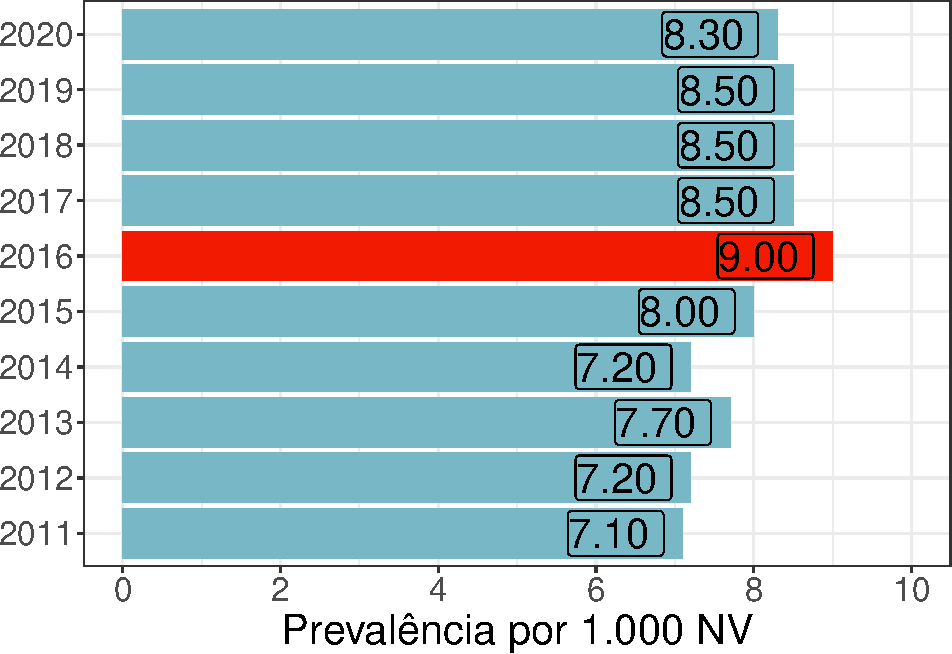
\includegraphics{anom_files/figure-latex/unnamed-chunk-28-1.pdf}

\hypertarget{por-ano-e-regiuxe3o}{%
\subsubsection{Por ano e região}\label{por-ano-e-regiuxe3o}}

\begin{Shaded}
\begin{Highlighting}[]
\NormalTok{dados\_nasc\_ano\_reg }\OtherTok{\textless{}{-}}\NormalTok{ dados\_nascidos }\SpecialCharTok{|\textgreater{}} 
  \CommentTok{\# selecionando os totais de nascidos por ano e regiao}
  \FunctionTok{filter}\NormalTok{(nivel }\SpecialCharTok{==} \StringTok{"região"}\NormalTok{ ) }\SpecialCharTok{|\textgreater{}} 
  \FunctionTok{select}\NormalTok{(}\SpecialCharTok{{-}}\NormalTok{nivel)}

\NormalTok{malf\_ano\_reg }\OtherTok{\textless{}{-}}\NormalTok{ d\_anom }\SpecialCharTok{|\textgreater{}} 
  \FunctionTok{mutate}\NormalTok{(}\AttributeTok{ano\_nasc =} \FunctionTok{as.character}\NormalTok{(ano\_nasc)) }\SpecialCharTok{|\textgreater{}} 
  \FunctionTok{rename}\NormalTok{(}\AttributeTok{local =}\NormalTok{ res\_REGIAO) }\SpecialCharTok{|\textgreater{}} 
  \FunctionTok{group\_by}\NormalTok{(ano\_nasc, local) }\SpecialCharTok{|\textgreater{}} 
  \CommentTok{\# contabilizando o numero de malformacoes por ano e regiao}
  \FunctionTok{summarise}\NormalTok{(}\AttributeTok{n\_casos =} \FunctionTok{sum}\NormalTok{(n\_malf))}

\NormalTok{malf\_ano\_reg }\OtherTok{\textless{}{-}}\NormalTok{ malf\_ano\_reg }\SpecialCharTok{|\textgreater{}} 
  \CommentTok{\# unindo os dados de anomalias com os dados de nascidos por ano e estado}
  \FunctionTok{left\_join}\NormalTok{(dados\_nasc\_ano\_reg, }\AttributeTok{by =} \FunctionTok{c}\NormalTok{(}\StringTok{"ano\_nasc"}\NormalTok{, }\StringTok{"local"}\NormalTok{)) }\SpecialCharTok{|\textgreater{}} 
  \CommentTok{\# criando percentual de casos de malformacoes por ano e estado}
  \FunctionTok{mutate}\NormalTok{(}
    \AttributeTok{local =} \FunctionTok{factor}\NormalTok{(local, }\AttributeTok{levels =} \FunctionTok{c}\NormalTok{(}\StringTok{"Norte"}\NormalTok{, }\StringTok{"Nordeste"}\NormalTok{, }\StringTok{"Centro{-}Oeste"}\NormalTok{, }\StringTok{"Sudeste"}\NormalTok{, }\StringTok{"Sul"}\NormalTok{)),}
    \CommentTok{\# calculando prevalencia por 1000 nv}
    \AttributeTok{prev =} \FunctionTok{round}\NormalTok{(n\_casos }\SpecialCharTok{/}\NormalTok{ total, }\DecValTok{4}\NormalTok{) }\SpecialCharTok{*} \DecValTok{1000}
\NormalTok{  )}
\end{Highlighting}
\end{Shaded}

\begin{Shaded}
\begin{Highlighting}[]
\FunctionTok{ggplot}\NormalTok{(malf\_ano\_reg, }\FunctionTok{aes}\NormalTok{(}\AttributeTok{x =}\NormalTok{ ano\_nasc, }\AttributeTok{y =}\NormalTok{ local, }\AttributeTok{fill =}\NormalTok{ prev)) }\SpecialCharTok{+}
  \CommentTok{\# mapa de calor}
  \FunctionTok{geom\_tile}\NormalTok{() }\SpecialCharTok{+}
  \FunctionTok{geom\_text}\NormalTok{(}\FunctionTok{aes}\NormalTok{(}\AttributeTok{label =} \FunctionTok{sprintf}\NormalTok{(}\StringTok{"\%.2f"}\NormalTok{, prev)), }\AttributeTok{color =} \StringTok{"\#000000"}\NormalTok{, }\AttributeTok{size =} \DecValTok{5}\NormalTok{) }\SpecialCharTok{+}
  \FunctionTok{theme\_bw}\NormalTok{() }\SpecialCharTok{+}
  \FunctionTok{scale\_fill\_gradientn}\NormalTok{(}\AttributeTok{colours =} \FunctionTok{wes\_palette}\NormalTok{(}\StringTok{"Zissou1"}\NormalTok{, }\DecValTok{100}\NormalTok{, }\AttributeTok{type =} \StringTok{"continuous"}\NormalTok{)) }\SpecialCharTok{+} 
  \FunctionTok{scale\_x\_discrete}\NormalTok{(}\AttributeTok{breaks =} \FunctionTok{seq}\NormalTok{(}\AttributeTok{from =} \DecValTok{2011}\NormalTok{, }\AttributeTok{to =} \DecValTok{2020}\NormalTok{, }\AttributeTok{by =} \DecValTok{1}\NormalTok{)) }\SpecialCharTok{+}
  \FunctionTok{labs}\NormalTok{(}\AttributeTok{y =} \StringTok{""}\NormalTok{, }\AttributeTok{fill =} \StringTok{"Prevalência }\SpecialCharTok{\textbackslash{}n}\StringTok{por 1.000 NV"}\NormalTok{) }\SpecialCharTok{+}
  \FunctionTok{theme}\NormalTok{(}
    \AttributeTok{text =} \FunctionTok{element\_text}\NormalTok{(}\AttributeTok{size =} \DecValTok{20}\NormalTok{),}
    \AttributeTok{axis.title.x =} \FunctionTok{element\_blank}\NormalTok{(),}
    \AttributeTok{legend.position =} \StringTok{"bottom"}\NormalTok{,}
    \AttributeTok{legend.key.width =} \FunctionTok{unit}\NormalTok{(}\DecValTok{2}\NormalTok{, }\StringTok{\textquotesingle{}cm\textquotesingle{}}\NormalTok{)}
\NormalTok{  )}
\end{Highlighting}
\end{Shaded}

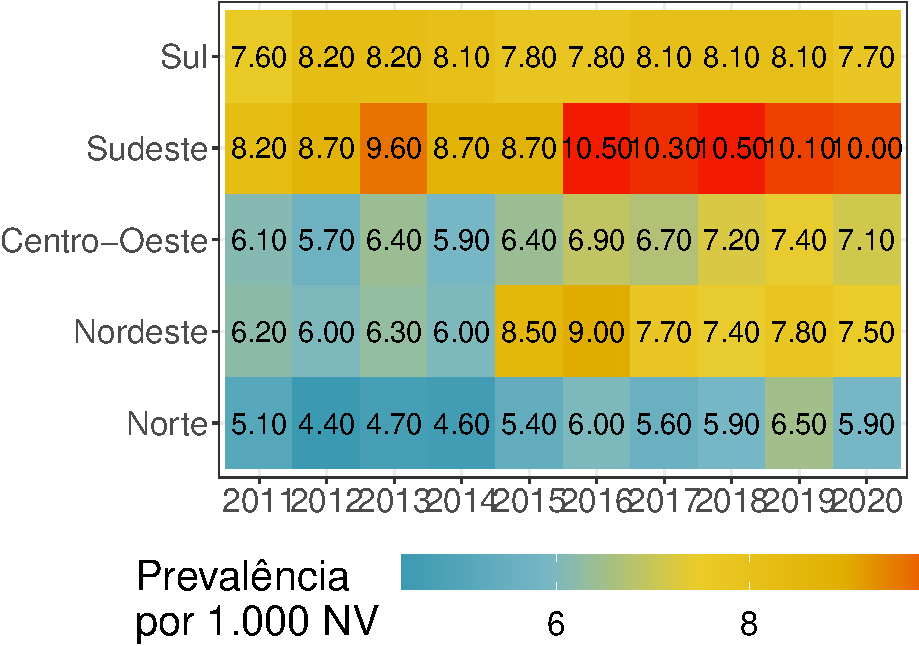
\includegraphics{anom_files/figure-latex/unnamed-chunk-30-1.pdf}

\hypertarget{por-ano-e-estado}{%
\subsubsection{Por ano e estado}\label{por-ano-e-estado}}

\begin{Shaded}
\begin{Highlighting}[]
\NormalTok{dados\_nasc\_ano\_uf }\OtherTok{\textless{}{-}}\NormalTok{ dados\_nascidos }\SpecialCharTok{|\textgreater{}} 
  \CommentTok{\# selecionando os totais de nascidos por ano e regiao}
  \FunctionTok{filter}\NormalTok{(nivel }\SpecialCharTok{==} \StringTok{"estado"}\NormalTok{ ) }\SpecialCharTok{|\textgreater{}} 
  \FunctionTok{select}\NormalTok{(}\SpecialCharTok{{-}}\NormalTok{nivel)}

\NormalTok{malf\_ano\_uf }\OtherTok{\textless{}{-}}\NormalTok{ d\_anom }\SpecialCharTok{|\textgreater{}} 
  \FunctionTok{mutate}\NormalTok{(}\AttributeTok{ano\_nasc =} \FunctionTok{as.character}\NormalTok{(ano\_nasc)) }\SpecialCharTok{|\textgreater{}} 
  \FunctionTok{rename}\NormalTok{(}\AttributeTok{local =}\NormalTok{ res\_NOME\_UF) }\SpecialCharTok{|\textgreater{}} 
  \FunctionTok{group\_by}\NormalTok{(ano\_nasc, local) }\SpecialCharTok{|\textgreater{}} 
  \CommentTok{\# contabilizando o numero de malformacoes por ano e regiao}
  \FunctionTok{summarise}\NormalTok{(}\AttributeTok{n\_casos =} \FunctionTok{sum}\NormalTok{(n\_malf))}

\NormalTok{malf\_ano\_uf }\OtherTok{\textless{}{-}}\NormalTok{ malf\_ano\_uf }\SpecialCharTok{|\textgreater{}} 
  \CommentTok{\# unindo os dados de anomalias com os dados de nascidos por ano e estado}
  \FunctionTok{left\_join}\NormalTok{(dados\_nasc\_ano\_uf, }\AttributeTok{by =} \FunctionTok{c}\NormalTok{(}\StringTok{"ano\_nasc"}\NormalTok{, }\StringTok{"local"}\NormalTok{)) }\SpecialCharTok{|\textgreater{}} 
  \FunctionTok{mutate}\NormalTok{(}
    \CommentTok{\# organizando os estados por regiao}
    \AttributeTok{local =} \FunctionTok{factor}\NormalTok{(}
\NormalTok{      local,}
      \AttributeTok{levels =} \FunctionTok{c}\NormalTok{(}
        \StringTok{"Rio Grande do Sul"}\NormalTok{, }\StringTok{"Santa Catarina"}\NormalTok{, }\StringTok{"Paraná"}\NormalTok{, }\CommentTok{\#s}
        \StringTok{"São Paulo"}\NormalTok{, }\StringTok{"Rio de Janeiro"}\NormalTok{, }\StringTok{"Espírito Santo"}\NormalTok{, }\StringTok{"Minas Gerais"}\NormalTok{, }\CommentTok{\#se}
        \StringTok{"Distrito Federal"}\NormalTok{, }\StringTok{"Goiás"}\NormalTok{, }\StringTok{"Mato Grosso"}\NormalTok{, }\StringTok{"Mato Grosso do Sul"}\NormalTok{, }\CommentTok{\#co}
        \StringTok{"Bahia"}\NormalTok{, }\StringTok{"Sergipe"}\NormalTok{, }\StringTok{"Alagoas"}\NormalTok{, }\StringTok{"Pernambuco"}\NormalTok{, }\StringTok{"Paraíba"}\NormalTok{, }
        \StringTok{"Rio Grande do Norte"}\NormalTok{, }\StringTok{"Ceará"}\NormalTok{, }\StringTok{"Piauí"}\NormalTok{, }\StringTok{"Maranhão"}\NormalTok{, }\CommentTok{\#ne}
        \StringTok{"Tocantins"}\NormalTok{, }\StringTok{"Pará"}\NormalTok{, }\StringTok{"Amapá"}\NormalTok{, }\StringTok{"Roraima"}\NormalTok{, }\StringTok{"Amazonas"}\NormalTok{, }\StringTok{"Rondônia"}\NormalTok{, }\StringTok{"Acre"} \CommentTok{\#n}
\NormalTok{      )}
\NormalTok{    ),}
    \CommentTok{\# calculando prevalencia por 1000 nv}
    \AttributeTok{prev =} \FunctionTok{round}\NormalTok{(n\_casos }\SpecialCharTok{/}\NormalTok{ total, }\DecValTok{4}\NormalTok{) }\SpecialCharTok{*} \DecValTok{1000}
\NormalTok{  )}
\end{Highlighting}
\end{Shaded}

\begin{Shaded}
\begin{Highlighting}[]
\FunctionTok{ggplot}\NormalTok{(malf\_ano\_uf, }\FunctionTok{aes}\NormalTok{(}\AttributeTok{x =}\NormalTok{ ano\_nasc, }\AttributeTok{y =}\NormalTok{ local, }\AttributeTok{fill =}\NormalTok{ prev)) }\SpecialCharTok{+}
  \CommentTok{\# mapa de calor}
  \FunctionTok{geom\_tile}\NormalTok{() }\SpecialCharTok{+}
  \FunctionTok{geom\_text}\NormalTok{(}\FunctionTok{aes}\NormalTok{(}\AttributeTok{label =} \FunctionTok{sprintf}\NormalTok{(}\StringTok{"\%.2f"}\NormalTok{, prev)), }\AttributeTok{color =} \StringTok{"\#000000"}\NormalTok{, }\AttributeTok{size =} \DecValTok{5}\NormalTok{) }\SpecialCharTok{+}
  \FunctionTok{theme\_bw}\NormalTok{() }\SpecialCharTok{+}
  \FunctionTok{scale\_fill\_gradientn}\NormalTok{(}\AttributeTok{colours =} \FunctionTok{wes\_palette}\NormalTok{(}\StringTok{"Zissou1"}\NormalTok{, }\DecValTok{100}\NormalTok{, }\AttributeTok{type =} \StringTok{"continuous"}\NormalTok{)) }\SpecialCharTok{+} 
  \FunctionTok{scale\_x\_discrete}\NormalTok{(}\AttributeTok{breaks =} \FunctionTok{seq}\NormalTok{(}\AttributeTok{from =} \DecValTok{2011}\NormalTok{, }\AttributeTok{to =} \DecValTok{2020}\NormalTok{, }\AttributeTok{by =} \DecValTok{1}\NormalTok{)) }\SpecialCharTok{+}
  \FunctionTok{labs}\NormalTok{(}\AttributeTok{y =} \StringTok{""}\NormalTok{, }\AttributeTok{fill =} \StringTok{"Prevalência }\SpecialCharTok{\textbackslash{}n}\StringTok{por 1.000NV"}\NormalTok{) }\SpecialCharTok{+}
  \FunctionTok{theme}\NormalTok{(}
    \AttributeTok{text =} \FunctionTok{element\_text}\NormalTok{(}\AttributeTok{size =} \DecValTok{20}\NormalTok{),}
    \AttributeTok{axis.title.x =} \FunctionTok{element\_blank}\NormalTok{(),}
    \AttributeTok{legend.position =} \StringTok{"bottom"}\NormalTok{,}
    \AttributeTok{legend.key.width =} \FunctionTok{unit}\NormalTok{(}\DecValTok{2}\NormalTok{, }\StringTok{\textquotesingle{}cm\textquotesingle{}}\NormalTok{)}
\NormalTok{  )}
\end{Highlighting}
\end{Shaded}

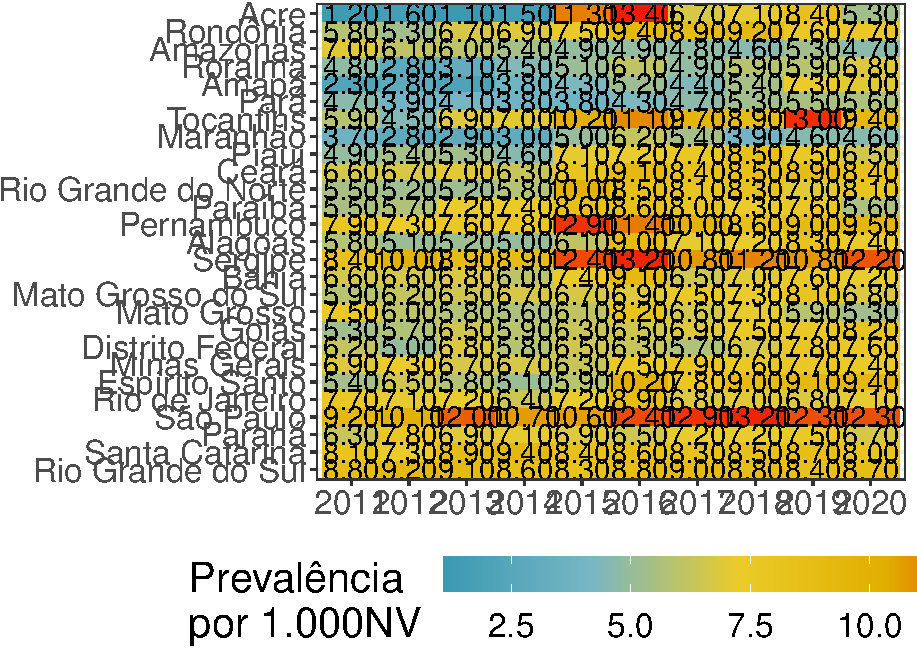
\includegraphics{anom_files/figure-latex/unnamed-chunk-32-1.pdf}

\newpage

\hypertarget{frequuxeancias-das-anomalias-conguxeanitas}{%
\section{8. Frequências das anomalias
congênitas}\label{frequuxeancias-das-anomalias-conguxeanitas}}

Nesta seção, encontram-se as tabelas de frequências e gráficos de barras
das malformações congênitas prioritárias, segundo grupos e subgrupos
definidos pela EUROCAT.

Para calcular as frequências (percentuais) das malformações congênitas,
foi feita a razão entre o número de ocorrência de cada malformação e o
total (soma) de ocorrência de todas as malformações. Para calcular as
frequências (percentuais) dos grupos de malformações congênitas, o
raciocínio foi análogo.

\hypertarget{tabela-de-frequuxeancias-para-as-malformauxe7uxf5es-conguxeanitas}{%
\subsubsection{Tabela de frequências para as malformações
congênitas}\label{tabela-de-frequuxeancias-para-as-malformauxe7uxf5es-conguxeanitas}}

Código omitido. Verificar no arquivo
\texttt{analise\_descritiva{[}2024-02-09{]}.Rmd} (linhas 1331-2309).

Resultado omitido. Foi gerado o arquivo \texttt{tab\_freqs.xlsx}.

\hypertarget{gruxe1fico-de-frequuxeancias-dos-grupos-de-malformauxe7uxf5es-conguxeanitas}{%
\subsubsection{Gráfico de frequências dos grupos de malformações
congênitas}\label{gruxe1fico-de-frequuxeancias-dos-grupos-de-malformauxe7uxf5es-conguxeanitas}}

\begin{Shaded}
\begin{Highlighting}[]
\NormalTok{readxl}\SpecialCharTok{::}\FunctionTok{read\_xlsx}\NormalTok{(}\StringTok{"02.analise/tab\_auxiliares/freqs\_cid10\_eurocat.xlsx"}\NormalTok{, }\AttributeTok{skip =} \DecValTok{1}\NormalTok{) }\SpecialCharTok{|\textgreater{}} 
  \FunctionTok{group\_by}\NormalTok{(grupo) }\SpecialCharTok{|\textgreater{}} 
  \FunctionTok{summarise}\NormalTok{(}\AttributeTok{n =} \FunctionTok{sum}\NormalTok{(n)) }\SpecialCharTok{|\textgreater{}}
  \FunctionTok{mutate}\NormalTok{(}
    \StringTok{\textasciigrave{}}\AttributeTok{\%}\StringTok{\textasciigrave{}} \OtherTok{=} \FunctionTok{round}\NormalTok{((n }\SpecialCharTok{/} \FunctionTok{sum}\NormalTok{(n)), }\DecValTok{4}\NormalTok{) }\SpecialCharTok{*} \DecValTok{100}\NormalTok{,}
    \AttributeTok{grupo =}\NormalTok{ forcats}\SpecialCharTok{::}\FunctionTok{fct\_reorder}\NormalTok{(grupo, }\SpecialCharTok{{-}}\StringTok{\textasciigrave{}}\AttributeTok{\%}\StringTok{\textasciigrave{}}\NormalTok{)}
\NormalTok{  ) }\SpecialCharTok{|\textgreater{}} 
  \FunctionTok{ggplot}\NormalTok{() }\SpecialCharTok{+}
    \FunctionTok{geom\_col}\NormalTok{(}\FunctionTok{aes}\NormalTok{(}\AttributeTok{x =}\NormalTok{ grupo, }\AttributeTok{y =} \StringTok{\textasciigrave{}}\AttributeTok{\%}\StringTok{\textasciigrave{}}\NormalTok{, }\AttributeTok{fill =}\NormalTok{ grupo)) }\SpecialCharTok{+} 
    \FunctionTok{labs}\NormalTok{(}\AttributeTok{y =} \StringTok{"Frequência (\%)"}\NormalTok{, }\AttributeTok{fill =} \StringTok{"Grupo:"}\NormalTok{) }\SpecialCharTok{+} 
    \FunctionTok{geom\_label}\NormalTok{(}
      \FunctionTok{aes}\NormalTok{(grupo, }\StringTok{\textasciigrave{}}\AttributeTok{\%}\StringTok{\textasciigrave{}}\NormalTok{, }\AttributeTok{label =} \FunctionTok{sprintf}\NormalTok{(}\StringTok{"\%.2f"}\NormalTok{, }\StringTok{\textasciigrave{}}\AttributeTok{\%}\StringTok{\textasciigrave{}}\NormalTok{), }\AttributeTok{fill =}\NormalTok{ grupo), }
      \AttributeTok{position =} \FunctionTok{position\_dodge}\NormalTok{(}\AttributeTok{width =}\NormalTok{ .}\DecValTok{9}\NormalTok{), }\AttributeTok{vjust =} \FloatTok{1.2}\NormalTok{, }\AttributeTok{size =} \DecValTok{7}\NormalTok{, }\AttributeTok{color =} \StringTok{"\#000000"}\NormalTok{, }
      \AttributeTok{show.legend =} \ConstantTok{FALSE}
\NormalTok{    ) }\SpecialCharTok{+}
    \FunctionTok{scale\_y\_continuous}\NormalTok{(}\AttributeTok{breaks =} \FunctionTok{seq}\NormalTok{(}\DecValTok{0}\NormalTok{, }\DecValTok{40}\NormalTok{, }\AttributeTok{by =} \DecValTok{5}\NormalTok{)) }\SpecialCharTok{+}
    \FunctionTok{scale\_fill\_manual}\NormalTok{(}\AttributeTok{values =} \FunctionTok{wes\_palette}\NormalTok{(}\StringTok{"Zissou1"}\NormalTok{, }\DecValTok{12}\NormalTok{, }\AttributeTok{type =} \StringTok{"continuous"}\NormalTok{)) }\SpecialCharTok{+}
    \FunctionTok{theme\_bw}\NormalTok{() }\SpecialCharTok{+}
    \FunctionTok{theme}\NormalTok{(}
      \AttributeTok{text =} \FunctionTok{element\_text}\NormalTok{(}\AttributeTok{size =} \DecValTok{20}\NormalTok{),}
      \AttributeTok{axis.title.x =} \FunctionTok{element\_blank}\NormalTok{(),}
      \AttributeTok{axis.text.x =} \FunctionTok{element\_blank}\NormalTok{(),}
      \AttributeTok{axis.ticks.x =} \FunctionTok{element\_blank}\NormalTok{(),}
      \AttributeTok{legend.position =} \StringTok{"bottom"}
\NormalTok{    )}
\end{Highlighting}
\end{Shaded}

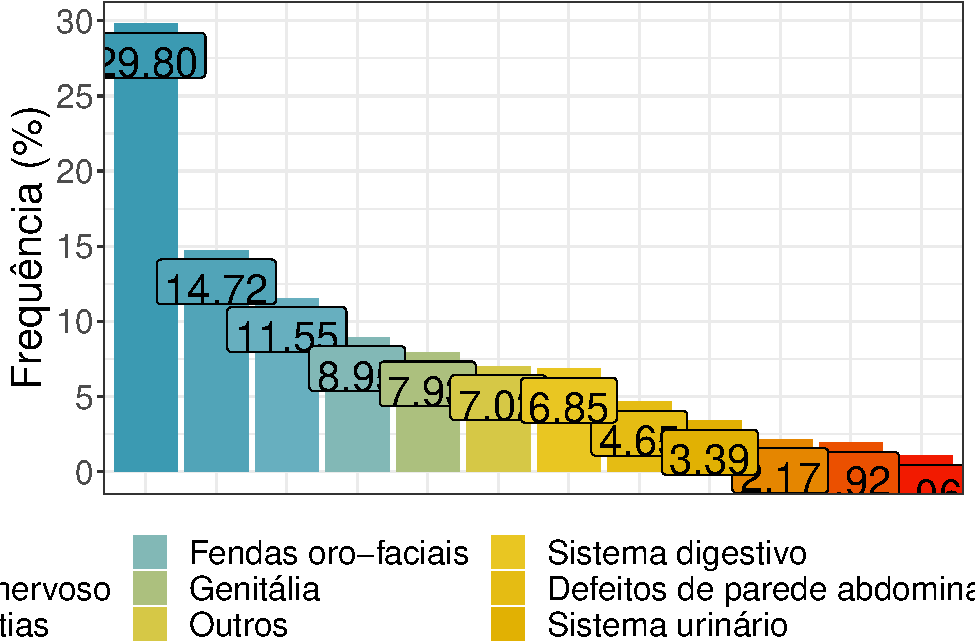
\includegraphics{anom_files/figure-latex/unnamed-chunk-35-1.pdf}

\hypertarget{gruxe1fico-de-frequuxeancias-das-10-malformauxe7uxf5es-conguxeanitas-mais-frequentes}{%
\subsubsection{Gráfico de frequências das 10 malformações congênitas
mais
frequentes}\label{gruxe1fico-de-frequuxeancias-das-10-malformauxe7uxf5es-conguxeanitas-mais-frequentes}}

\begin{Shaded}
\begin{Highlighting}[]
\NormalTok{tab\_cid10 }\SpecialCharTok{|\textgreater{}} 
  \FunctionTok{slice}\NormalTok{(}\DecValTok{1}\SpecialCharTok{:}\DecValTok{10}\NormalTok{) }\SpecialCharTok{|\textgreater{}} 
  \FunctionTok{mutate}\NormalTok{(}
    \AttributeTok{cid10 =}\NormalTok{ forcats}\SpecialCharTok{::}\FunctionTok{fct\_reorder}\NormalTok{(cid10, }\SpecialCharTok{{-}}\FunctionTok{as.numeric}\NormalTok{(}\StringTok{\textasciigrave{}}\AttributeTok{\%}\StringTok{\textasciigrave{}}\NormalTok{)),}
    \AttributeTok{categoria =}\NormalTok{ forcats}\SpecialCharTok{::}\FunctionTok{fct\_reorder}\NormalTok{(categoria, }\SpecialCharTok{{-}}\FunctionTok{as.numeric}\NormalTok{(}\StringTok{\textasciigrave{}}\AttributeTok{\%}\StringTok{\textasciigrave{}}\NormalTok{))}
\NormalTok{  ) }\SpecialCharTok{|\textgreater{}}
  \CommentTok{\# grafico de barras}
  \FunctionTok{ggplot}\NormalTok{() }\SpecialCharTok{+}
    \FunctionTok{geom\_col}\NormalTok{(}\FunctionTok{aes}\NormalTok{(}\AttributeTok{x =}\NormalTok{ cid10, }\AttributeTok{y =} \FunctionTok{as.numeric}\NormalTok{(}\StringTok{\textasciigrave{}}\AttributeTok{\%}\StringTok{\textasciigrave{}}\NormalTok{), }\AttributeTok{fill =}\NormalTok{ categoria)) }\SpecialCharTok{+} 
    \FunctionTok{labs}\NormalTok{(}\AttributeTok{x =} \StringTok{"CID{-}10"}\NormalTok{, }\AttributeTok{y =} \StringTok{"Frequência (\%)"}\NormalTok{, }\AttributeTok{fill =} \StringTok{"Descrição:"}\NormalTok{) }\SpecialCharTok{+} 
    \FunctionTok{geom\_label}\NormalTok{(}
      \FunctionTok{aes}\NormalTok{(cid10, }\FunctionTok{as.numeric}\NormalTok{(}\StringTok{\textasciigrave{}}\AttributeTok{\%}\StringTok{\textasciigrave{}}\NormalTok{), }\AttributeTok{label =} \FunctionTok{sprintf}\NormalTok{(}\StringTok{"\%.2f"}\NormalTok{, }\FunctionTok{as.numeric}\NormalTok{(}\StringTok{\textasciigrave{}}\AttributeTok{\%}\StringTok{\textasciigrave{}}\NormalTok{)), }\AttributeTok{fill =}\NormalTok{ categoria), }
      \AttributeTok{position =} \FunctionTok{position\_dodge}\NormalTok{(}\AttributeTok{width =}\NormalTok{ .}\DecValTok{9}\NormalTok{), }\AttributeTok{vjust =} \FloatTok{1.2}\NormalTok{, }\AttributeTok{size =} \DecValTok{7}\NormalTok{, }\AttributeTok{color =} \StringTok{"\#000000"}\NormalTok{, }
      \AttributeTok{show.legend =} \ConstantTok{FALSE}
\NormalTok{    ) }\SpecialCharTok{+}
    \FunctionTok{scale\_y\_continuous}\NormalTok{(}\AttributeTok{breaks =} \FunctionTok{seq}\NormalTok{(}\DecValTok{0}\NormalTok{, }\DecValTok{10}\NormalTok{, }\AttributeTok{by =} \DecValTok{2}\NormalTok{)) }\SpecialCharTok{+}
    \FunctionTok{scale\_fill\_manual}\NormalTok{(}\AttributeTok{values =} \FunctionTok{wes\_palette}\NormalTok{(}\StringTok{"Zissou1"}\NormalTok{, }\DecValTok{10}\NormalTok{, }\AttributeTok{type =} \StringTok{"continuous"}\NormalTok{)) }\SpecialCharTok{+}
    \FunctionTok{theme\_bw}\NormalTok{() }\SpecialCharTok{+}
    \FunctionTok{theme}\NormalTok{(}
      \AttributeTok{text =} \FunctionTok{element\_text}\NormalTok{(}\AttributeTok{size =} \DecValTok{20}\NormalTok{),}
      \AttributeTok{legend.position =} \FunctionTok{c}\NormalTok{(.}\DecValTok{82}\NormalTok{, .}\DecValTok{8}\NormalTok{),}
      \AttributeTok{legend.background =} \FunctionTok{element\_rect}\NormalTok{(}\AttributeTok{linetype =} \StringTok{"solid"}\NormalTok{, }\AttributeTok{colour =} \StringTok{"\#000000"}\NormalTok{)}
\NormalTok{    )}
\end{Highlighting}
\end{Shaded}

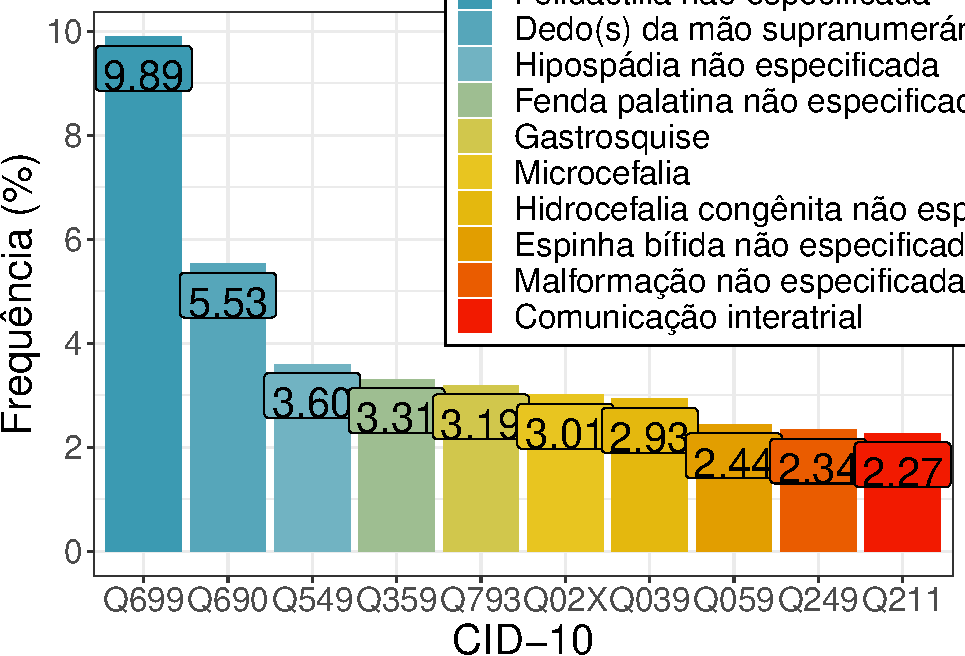
\includegraphics{anom_files/figure-latex/unnamed-chunk-36-1.pdf}

\newpage

\hypertarget{tabela-e-gruxe1ficos-de-prevaluxeancias-dos-grupos-de-anomalias-conguxeanitas}{%
\section{9. Tabela e gráficos de prevalências dos grupos de anomalias
congênitas}\label{tabela-e-gruxe1ficos-de-prevaluxeancias-dos-grupos-de-anomalias-conguxeanitas}}

Nesta seção, encontram-se a tabela de prevalência de malformações
congênitas prioritárias, segundo grupos definidos pela EUROCAT e
características maternas, da gestação, do parto e do recém-nascido, e os
mapas geográficos representativos da distribuição das prevalências
desses grupos, por estado de residência da mãe.

Para calcular as prevalência dos grupos de malformações congênitas, foi
feita a razão entre o número de ocorrência de cada grupo e o total de
nascidos vivos (NV) registrados no período analisado multiplicado por um
fator de 1.000 NV. Para calcular as prevalências dos grupos de
malformações congênitas a nível estadual, o raciocínio foi análogo,
porém considerando o total de NV no período analisado e estado.

\hypertarget{tabela-de-prevaluxeancia-dos-grupos-de-malformauxe7uxf5es-conguxeanitas}{%
\subsubsection{Tabela de prevalência dos grupos de malformações
congênitas}\label{tabela-de-prevaluxeancia-dos-grupos-de-malformauxe7uxf5es-conguxeanitas}}

Código omitido. Verificar no arquivo
\texttt{analise\_descritiva{[}2024-02-09{]}.Rmd} (linhas 2458-2813).

Resultado omitido. Foi gerado o arquivo \texttt{tab\_prevs.xlsx}.

\hypertarget{mapas-da-distribuiuxe7uxe3o-de-prevaluxeancia-dos-grupos-de-malformauxe7uxf5es-conguxeanitas}{%
\subsubsection{Mapas da distribuição de prevalência dos grupos de
malformações
congênitas}\label{mapas-da-distribuiuxe7uxe3o-de-prevaluxeancia-dos-grupos-de-malformauxe7uxf5es-conguxeanitas}}

Código omitido. Verificar no arquivo
\texttt{analise\_descritiva{[}2024-02-09{]}.Rmd} (linhas 2742-3002).

Resultado omitido. Foi gerado o arquivo \texttt{g\_map.png}.

\end{document}
